\part{The Robot Observer} % Main chapter 
\label{part:robot_observer} % Change X to a consecutive number; for referencing this chapter elsewhere, use \ref{ChapterX}

\lhead{Part II. \emph{The Robot Observer}} % Change X to a consecutive number; this is for the header on each page - perhaps a


In any application that is not entirely composed by repetitive, precomputed actions, robots need reasoning skills, which severely depend on the quality of the representation of the current environment. This representation can be more or less complex, depending on the application. 

Imagine, for example, a robot whose task is cleaning the floor of a room. In the simplest case, this robot would only be provided with an elementary set of sensors. Without the capacity to understand which areas actually need cleaning, this robot could only move through the room, randomly or with some strategy, achieving the task in a longer amount of time than what would actually be needed. 

% In a fairly simple case, this robot would rely on a map of the room and a set of lasers, or bumper sensors, to detect obstacles. 

Now, imagine a household robot that needs to actively help a family that lives in an apartment, by fetching objects, providing information, and helping to accomplish various tasks. Let us imagine that one of the members of the family, Greg, is moving in the living room, searching around, while exclaiming `Where are my glasses?'. In the ideal situation, our robot would try to help Greg, by giving him information such as `They are on the table to your right', or even by fetching them for him. 

Clearly, in this scenario, the robot needs deeper reasoning skills. It needs to understand that the user is looking for its glasses, to link them to their actual physical location, to compute the spatial relationship between the table and the glasses, and to provide information in a natural way. In fact, if the robot would tell Greg that the glasses are in the position $(3.2, 5.0 , 1.3)$, Greg would likely be very perplexed. A more natural way would be to inform Greg that his glasses are on a table, whose location is pointed taking into account Greg's position.

In this case, having sophisticated sensors is, of course, important but not sufficient. The robot needs also to \textit{reason} on the sensor's data in order to produce meaningful information. For example: laser points and camera images need to be integrated to recognize objects and humans; spatial relationships  (e.g. the glasses are on the table) have to be properly modeled; actions performed by humans, and their effects on the environment, need to be recognized; and so on. 

The process of reasoning on data to produce symbolic information is called \textit{situation assessment}. Endsley explained in \cite{endsley1995toward} that this process is deeply linked to the quality of  decisions of the robot.

While in many applications robots can benefit from a situation assessment component, being able to perform complex reasoning on data is particularly important in HRI. If the robot is able to take better decisions (i.e.  efficient, safe, socially acceptable, natural) than it will be perceived in a more positive manner by humans. 

Situation assessment is the fundamental skill for the \textit{robot observer}. In this part, we will show the situation assessment mechanisms of our system. Chapter~\ref{chapter:belief_management} shows how we can use geometrical reasoning in order to understand what the robot and other humans know and perceive about the current environment. Chapter~\ref{chapter:intention} shows how our robot is able to infer the current intention of a human and the actions it performs. Finally, chapter~\ref{chapter:observer_results} details a user study that we developed to validate our intention recognition algorithm.



                 % Chapter Template

\chapter{Belief Management} % Main chapter title

\label{chapter:belief_management} % Change X to a consecutive number; for referencing this chapter elsewhere, use \ref{ChapterX}

\lhead{Chapter 3. \emph{Belief Management}} % Change X to a consecutive number; this is for the header on each page - perhaps a shortened title

In this chapter we show how our system is able to manage agents beliefs. Section~\ref{sec:belief_management-intro} provides an introduction to the subject, with a discussion on some relevant works. Section~\ref{sec:belief_management-overview} shows an overview of our approach, discussing its key aspects and modules. Sections~\ref{sec:belief_management-system_inputs}  shows the simplified mechanism that we use to detect objects and humans. In section~\ref{sec:belief_management-geometrical_reasoning} we explain the geometrical reasoning capacities of our system, introducing the main symbolic facts that are computed. Finally, in section~\ref{sec:belief_management-belief_management} we show how we build human belief models starting from these facts.

\section{Introduction}
\label{sec:belief_management-intro}
%Motivation

In HRI, it is important to represent humans not as simple obstacles, but as acting entities, with different beliefs on the state of the world and with the capacity to affect the environment. 

A simple example to prove this point is related to proxemics. Normally, when we approach an object, like a table, in an empty environment, we just choose the quickest path. If, intead, the environment is populated by other people, we will follow a set of social rules, like keeping a certain distance from them. If the robot does not follow these rules, it might freighten people, for example by approaching quickly from behind the person, or be considered as `rude'.


Theory of Mind~\citep{premack1978does} is a skill used to reason about humans' beliefs and thoughts, and how they affect actions. An ability linked to this concept is perspective taking, which is widely studied in developmental literature.  Flavell in \cite{flavell1977development} describes two levels of perspective taking: 
perceptual perspective taking, the capacity to understand that other people see the world differently \citep{Tversky1999}; and conceptual perspective taking, the capacity to attribute thoughts and feelings to other people \citep{Baron1985}. 

Through perceptual perspective taking we are able to compute information such as `I can see the glasses, but you can not', `you can reach the bottle, but I can not'. Conceptual perspective taking is equally important, and allows us, for example, to understand that a friend, when choosing the flavors for its ice cream, would choose its favourites, which might differs from ours.

An important study linked to conceptual perspective taking is the \textit{divergent belief task}.  Formulated in~\cite{wimmer1983}, this kind of task requires the ability to recognize that others can have beliefs about the world that differ from the observable reality.  A typical test used to study divergent belief is the Sally and Anne test (Figure~\ref{fig:belief_management-sally_anne}). In this test, Sally and Anne are two puppets. A short scene is shown to participants, where Sally takes a ball and hides it in her basket, before leaving the room. While she is away, Anne takes the ball from Sally's basket and puts it in her  box. After Sally returns, participants are asked a question: ``Where will Sally look for her object?''. Young children, or those affected by autism, might answer (wrongly) that Sally will look for her object in Anne's box, not taking into account that she does not know that it was moved.

 \begin{figure}[ht!]
	\centering
	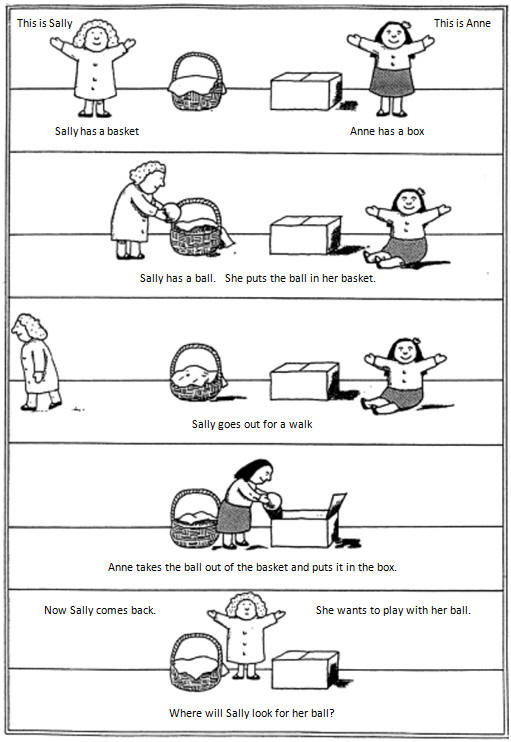
\includegraphics[scale=0.45]{img/observer/sally-anne.jpg}
	\caption{The Sally and Anne test. Original artwork by Axel Scheffler.}
	\label{fig:belief_management-sally_anne}
\end{figure}

Studies on individuals that do not possess the required mechanisms to perform perspective taking \citep{frick2014picturing} have shown that they encounter great difficulties in social relationships, confirming the importance of this ability.

These studies make us think that perspective taking could be very important in robotics. For example, let us imagine a scenario where Greg and a robot are performing some household repairs, which require the use of different tools. The robot might create a plan to achieve this goal where the human needs to use a screwdriver, which is actually behind a box, hidden from the sight of  Greg. Without perspective taking, the robot will procede in its task while Greg is desperately looking for the screwdriver. By using perspective taking, instead, the robot would infer that Greg does not know where the screwdriver is, and can not see it. In this situation, the robot might inform Greg of the location of the screwdriver, give it to him, or create a plan where Greg does not need to use it, thus being a more likable helper.

Previous works in robotics have actually demonstrated that enhancing the robot's perspective taking abilities improves its reasoning capabilities, leading to more appropriate and efficient task planning and interaction strategies \citep{Trafton2005,ros2010one,breazeal2006}. Let us review some implementations of perspective taking.

The HAMMER system, previously presented in chapter~\ref{chapter:introduction}, has been extended in~\cite{johnson2005perceptual} to introduce perceptual perspective taking, using the concept of forward and inverse visual models. Forward vision models analyze sensory data to produce information, like the geometrical coordinates of objects. Inverse visual models, instead, receive as input desired properties and states (for example, the presence of objects of a certain shape and color in a particular location), and try to produce an appropriate visual image that respects these inputs.

Perspective taking is performed by introducing two forward vision models. The first one produces the location and relationships between objects and end effectors (like grippers), while the second  computes the gaze direction of other agents. Using the results of these models as input of an inverse visual model, the system can reconstruct the scene as seen by another agent. The representation of knowledge by agents is not explicitly handled in the system. 

The architecture of~\cite{BreazealGB09}, also presented in chapter~\ref{chapter:introduction}, is another cognitive system which uses simulation mechanisms, but the work  includes both perceptual and conceptual perceptive taking. In this system the robot's schemas are used to build its mental model and execute its tasks, but also to build humans mental models and infer their actions and goals.

The robot is able to build a belief on the world state by analyzing perceptual data, producing symbolic information, such as the location or color of an object. This belief is constantly maintained, by adding new information and erasing those that are no longer valid.

To build a belief model of a human, the robot manipulates perceptual data, by filtering objects that can not be seen by the human (because they are occluded, for example), and transforming the data to simulate a first-person experience on the human. By using the same mechanisms to manage the belief for itself and for humans, the robot can infer divergent belief situations. This method has been tested on variants of the Sally and Anne test with good results.

The belief management algorithm of this systems does not take into account information that can not be directly perceived, but must be inferred. For example, in a domestic scenario, a human might not be aware that a mug containing liquid is hot and should not be touched. These aspects could be inferred by taking into account the results of actions, like pouring hot liquid in the mug.

Another system able to model agent beliefs is~\cite{scheutz2013computational}. This work is oriented toward problems where a distributed team of agents needs to communicate over a remote connection to solve a task. Each agent is assumed to be able to create its own mental model using its perception capacities, even though the precise rules for these mechanisms are not explained. When an agent receives information, he updates his mental belief using a set of rules, introducing the new data and checking for incongruencies with his previous information.  Using the same mechanism, each agent forms a belief model of other agents that have received the same information.

We created a rule-based approach for belief management, based on geometric reasoning and on inference, which we will introduce in the following sections. 

\section{Belief Management Overview}
\label{sec:belief_management-overview}

\subsection{Process overview}

Managing beliefs means being able to build and maintain a model of the belief of each agent. Our system is able to accomplish this task with different steps.

Of course, to reason on the current situation the system needs to be able to detect humans and objects in the environment. In some case, to be generic, we will call an agent or an object an \textit{entity}. Section~\ref{belief_management:entity_detection} will show how detect and track entities.

We can assign \textit{attributes} to entities, parts of entities (e.g. the arm of a human), and areas to represent different information, like properties, the state of entities or relationships between entities. Examples of attributes are:
an agent can be in a specific area; a box can be opened and can contain objects; a bottle can contain liquids; a mug can be hot; a room can be a silent area, where the robot should avoid making any noise.
We divide attributes in two classes, which influence the capacity of agents to perceive them: 
\begin{itemize}
\item Fully observable. These attributes can be observed by any present agent looking at the linked entity or area (e.g. the box is open, Greg is in the kitchen).
\item Partially observable. These attributes can be observed by present agents only in specific situations, represented as rules linked to the object and the attributes, e.g. an agent can see that a box contains items only when it is open, an agent can detect that the mug is hot only when he touches it. 
\end{itemize}

The locations of entities are integrated with other data produced by sensors through geometrical reasoning in order to produce symbolic informations, such as spatial relationships between objects and humans. We represent these information as facts. A fact is a tuple $subject\> predicate\> value$, which we use to represent symbolic knowledge. An example of fact is $CUP\> isOn\> TABLE$, which defines the location of an object. The instance of an attribute is represented as a fact, and so, each fact will correspond to exactly one attribute. More details about this aspect will be shown in section~\ref{sec:belief_management:geometrica_reasoning}.

We call \textit{world state} the collection of all facts describing the current situation. A \textit{belief model} is a collection of facts representing the knowledge of an agent on the world state. Each agent can have a different belief model, since the environment can change without an agent being able to perceive it. To represent the lack of knowledge of an agent, the value of a property can be \textit{unknown}. For example, the robot could take a tool from the table, while Greg is in another room, and place it in a box. Greg has not seen this event, and so his belief model will contain the (wrong) information that the tool is still on the table.  Section~\ref{sec:belief_management-belief_management} will show in, details, our approach to update the belief model of an agent.

In general, beliefs models are updated when the system infers that an \textit{action} has been executed, bringing a change to the environment.  We define an action as a tuple $(name, preconditions, target, postconditions)$. The $name$ of an action is a unique string that identifies it. The $preconditions$ are a set of facts that must be true in order to realize the action. In our system, an action is executed on a $target$, which can be a physical object, like a cup, but also an area of the environment, like a room. The $postconditions$ are the set of facts, and their values, affected by the action's execution.  


Since we are interested on reasoning and not perceptual aspects, we use inference, as explained in section \ref{sec:belief_management-intention_recognition}, in order to understand when a human has performed an action. Through the predefined $postconditions$ of actions we can also infer changes in the state of objects, e.g. the human opens a box, so the box is now open. 


\subsection{Architecture}
These aspects are represented in the Situation Assessment layer, and in particular in the following modules, shown in figure~\ref{fig:belief_management-belief_management_overview}.

\begin{itemize}
\item Sensor Data. Data produced by different possible sensors (e.g. lasers, camera, etc.).
\item Entity Detection. Different components detect and track humans and objects in the environment.
\item Geometrical Reasoning. Symbolic facts are produced starting from perceptual data.
\item Belief Management. The system maintains a mental model of each agent.
\item Database. The Database stores symbolic facts produced by the system.
\item Intention and Action Recognition. The system infers the current intentions of a human, and which actions are executed, by integrating  geometrical reasoning, the human's belief model, planning, and bayesian inference.
\end{itemize}

 \begin{figure}[ht!]
	\centering
	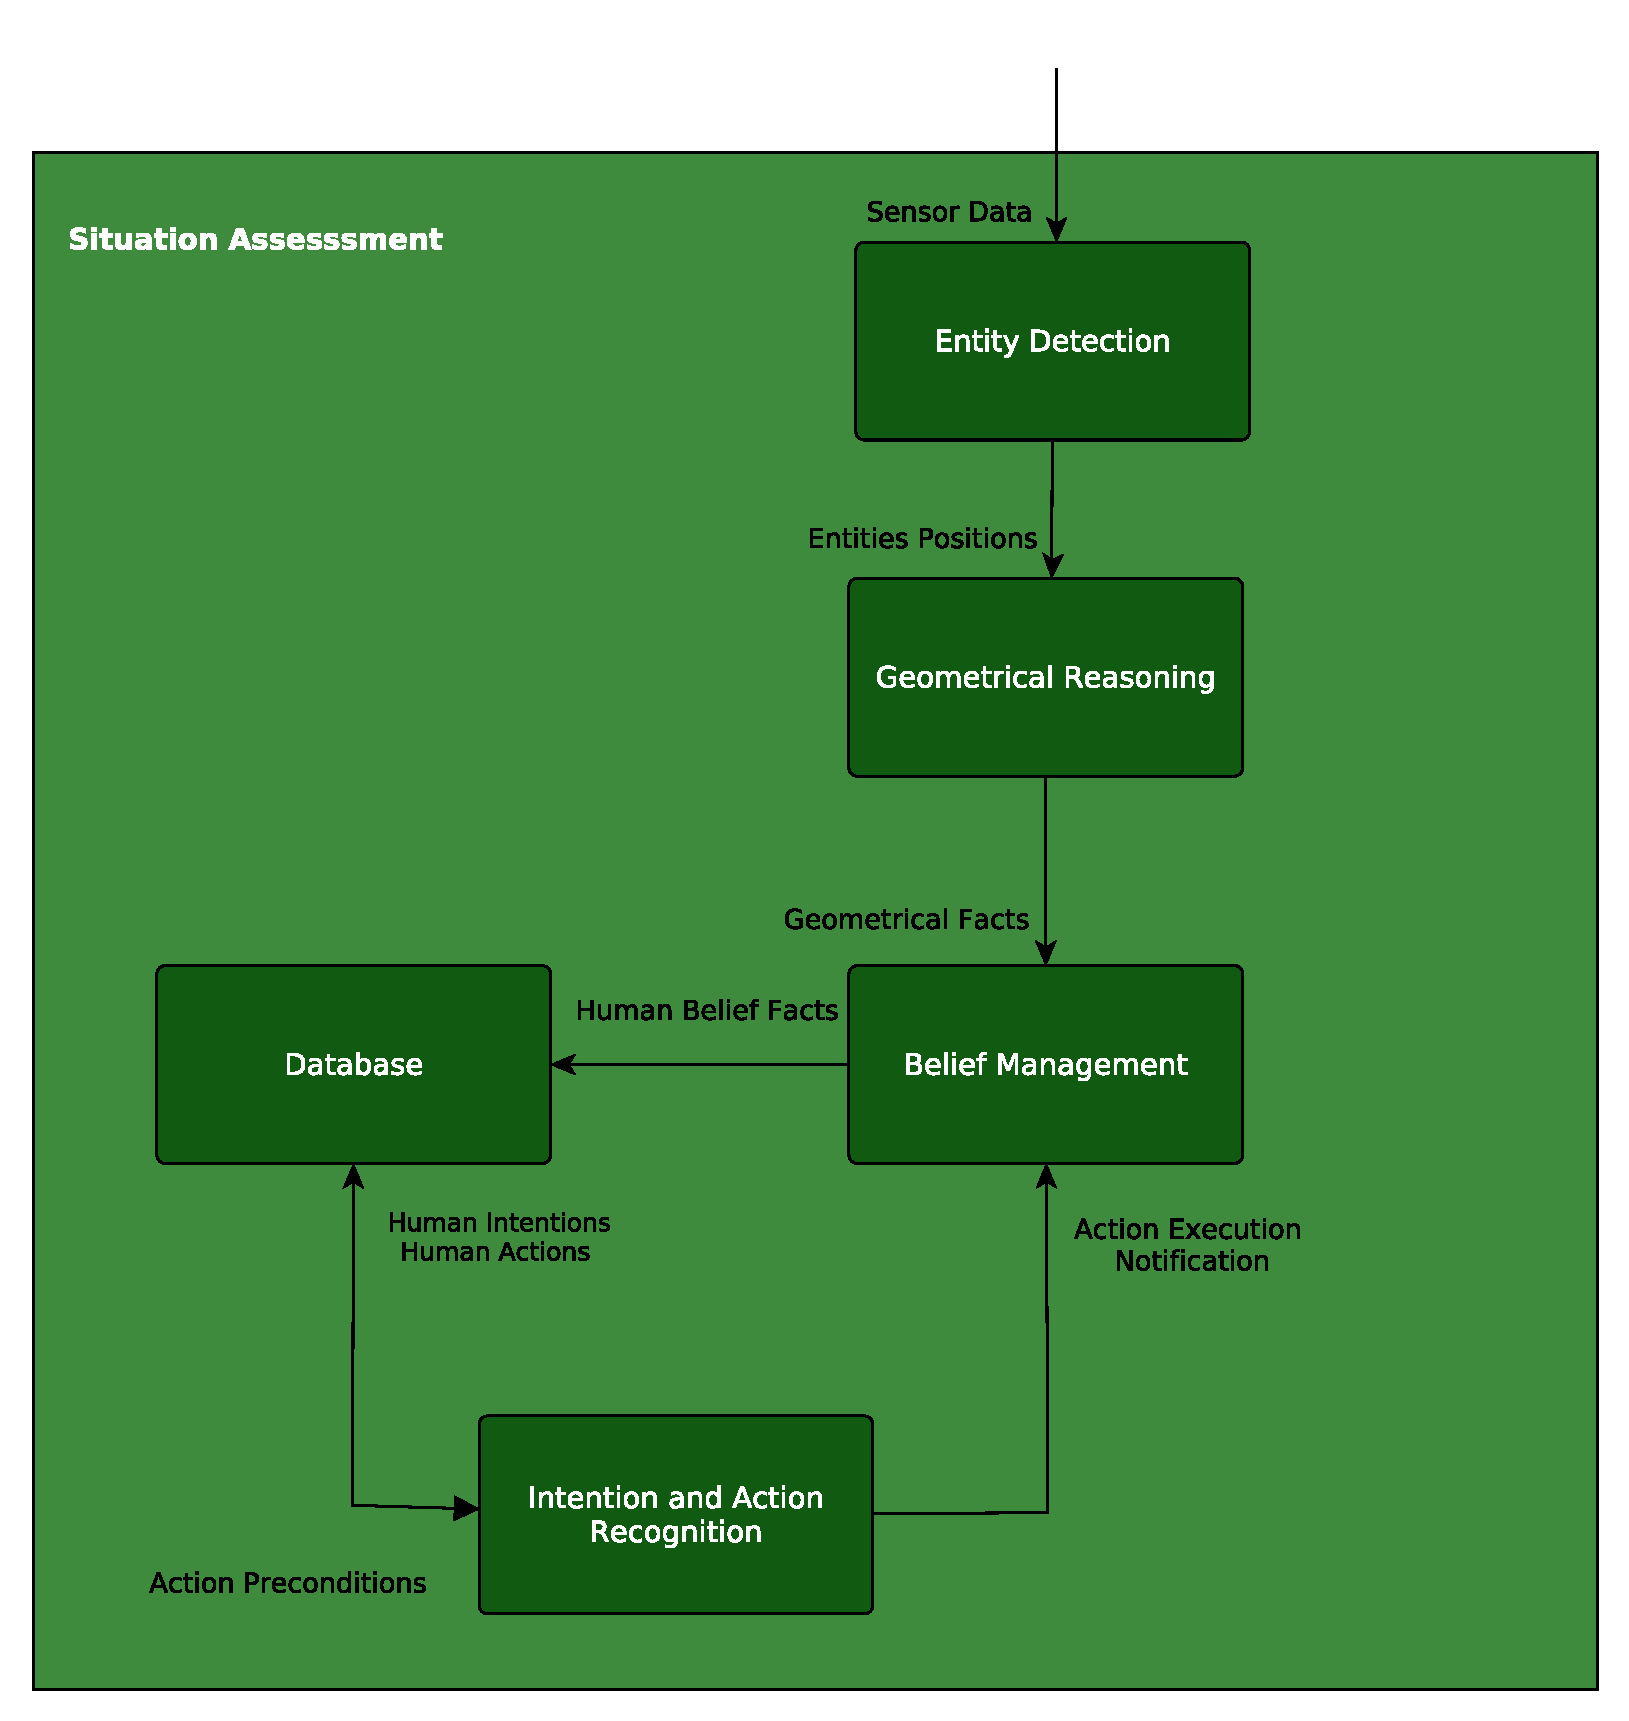
\includegraphics[scale=0.45]{img/observer/situation_assessment_overview.pdf}
	\caption{Overview of the different modules composing the Situation Assessment layer}
	\label{fig:belief_management-belief_management_overview}
\end{figure}

Symbolic facts are constantly produced, starting from the sensor data and from the position of entities. The Belief Manager collects these information to maintain the belief model of each agent. The belief model of humans and of the robot is used by the Intention and Action Recognition module to infer the most likely human intentions, and which actions they perform. All these information are introduced in the Database, and can be read by other components. For example, the Goal Management layer can choose a goal based on human commands or an estimation of humans' intentions. In a similar way, the Task Execution layer will read the Database in order to obtain the state of the world, to check action preconditions.  

The geometrical reasoning and belief management capacities of this layer were presented in \cite{Milliez2014}, where they were used to pass the Sally and Anne test~\cite{Baron1985} on a robotic platform. 

Dialogue can be a very important source of information. Agents often communicate, while executing a task together, or even when working independently, to clarify ambiguities and obtain missing information. While we will not present a specific dialogue component in this work,  in \cite{Ferreira2015} our belief management component was integrated with a situated dialogue system in a simulator. This model was compared with a basic system (without belief awareness) in a study with 60 interactions, in a simulated environment. We successfully showed that the dialogue management system significantly improves its efficiency, reducing the number of dialogue turns in the interaction, and its accuracy, with a higher success rate when a divergent belief situation appears.

In the following sections we will show how our system is able to manage agents' belief models. Actions will be treated, at this point, as input received by the Belief Management module. The intention and action recognition capacities of our system will be explained in~\ref{chapter:intention_recognition}. 

\section{Entity Detection}
\label{sec:belief_management-entity_detection}
In our system, we chose to simplify perception issues, focusing on reasoning aspects. We associate a unique tag to every object that is interesting in a particular scenario. When the robot observes a tag using a camera, it detects the corresponding object using a tag-matching algorithm.
Regarding humans, we use a motion capture software to identify and track agents moving in the environment. Using different tags, we can track the head, shoulders, and right arm of a human. Our situation assessment component has also been tested using a laser and RGB based detector, detailed in~\cite{lindermulti}, in the SPENCER european project. We also experimented using a depth camera, mounted on the ceiling, and a color-recognition algorithm to identify humans. 

 \begin{figure}[ht!]
	\centering
	\includegraphics[scale=0.7, trim={0 3cm 0 0}]{img/observer/explore.pdf}
	\caption[The robot builds a representation of the environment]{The robot explores the environment, recognizing objects through tags, and building a representation of the environment.}
	\label{fig:belief_management-explore}
\end{figure}

\section{Geometrical Reasoning}
\label{sec:belief_management-geometrical_reasoning}

Using its perception abilities the robot can build a representation of the environment, starting with entities' positions. With geometrical reasoning we can compute spatial relationships between entities, e.g. the glasses are on the shelf, the human is moving toward the library, the glasses are reachable by the human, the bottle is visible for the human. These reasonings provide a base for the perspective taking abilities of the robot.  The geometrical reasoning capacities of our system were introduced in~\cite{Sisbot2011}. This work was updated to include the production of new symbolic facts. We will show a list of some of the most important facts that our system is able to produce through geometrical reasoning.

\begin{itemize}
\item \textit{isOn}. Used when an object is on top of another, for example $CUP\; isOn\; TABLE$.
\item \textit{isNextTo}. Used when two objects are on the same surface and close to each other, for example $CUP\; isNextTo\; BOX$.
\item \textit{isReachable}. Used when an object is reachable by an agent, computed through inverse kinematics. An example of such predicate is $CUP\; isReachableBy\; ROBOT$
\item \textit{isVisible}. Used when an entity is visible by an agent. This is calculated by computing the field of view of an agent, and checking if there is a sufficient portion of the object not hidden by occlusions in this field. An example of this predicate is $CUP\; isVisibleBy\; ROBOT$.
\item \textit{isMoving}. Used when an agent is currently moving. This is computed by checking if the agent's displacements in a pre-determined time unit is bigger than a pre-determined threshold. We use an hysteresis filter to avoid continuous oscillation in the value of the fact. An example of $isMoving$ is $ROBOT\; isMoving\; TRUE$.
\item \textit{isMovingToward}. Used to indicate that an agent is moving toward a particular entity. This is computed by checking if the distance between the agent and the entity is decreasing. An example of this predicate is $ROBOT\; isMovingToward\; GREG$.
\item \textit{isOrientedToward}. Used to indicate that an agent is oriented toward a particular entity, for example $ROBOT\; isOrientedToward\; GREG$.
\item \textit{pose}. Used to indicate that an agent is in a particular pose, for example $GREG\; pose\; HANDOVER$.
\item \textit{isAt}. Used to indicate that an agent is in a particular location, for example $GREG\; isAt\; LIVING\_ROOM$.
\end{itemize}


\section{Belief Management}
\label{sec:belief_management-belief_management}
We have created a rule based framework in order to build the beliefs of each agent and update them when needed. Human belief models are updated using the perspective taking skills of the robot. When the robot detects the execution of an action in the world, with the mechanisms shown in chapter~\ref{chapter:intention_recognition},
it updates the belief model for itself and for every human that can perceive the action, adding its $postconditions$ to their models. When an action is not perceived by a human (e.g. the user was in another room), his belief model will not be updated, as he is not aware of the changes that occurred.

However, when he comes back and looks at the environment, we assign him a new belief state following a set of rules, which we will now explain. We call $p$ a fact, $H$ the agent, $HB$ his belief model, and $RB$ the robot's belief model. We also create the following predicates: $obs(p)$ means that $p$ is observable for $H$, $valid(p,x)$ means that $p$ does not contradict the current perception data of agent $x$, $value(p,m)$ is the value $p$ in belief model $m$, and $vis(p,x)$ means that agent $x$ has visibility on the linked entities of $p$ (e.g. if $p$ is $MUG\; isOn \; TABLE$ the linked entities are $MUG$ and $TABLE$) . The rules for the $valid$ predicate will be different in each attribute. For example the fact \textit{MUG isOn TABLE} will not be valid for agent Max if he can see that there is no mug on the table. For each fact $p\in HB \cup RB$:
\begin{itemize}
\item if $p \in RB, \quad p\not\in HB,\quad obs(p),\quad vis(p,H) \rightarrow value(p,HB)=value(p,RB)$.
\item if $p \not \in RB,\quad p\in HB,\quad obs(p),\quad vis(p,H) \rightarrow remove\quad $p$ \quad from \quad HB$.
\item if $p\in RB,\quad p\in HB$ then:
	\begin{itemize}
      \item if $value(p,HB)\neq value(p,RB),\\ \quad obs(p),\quad vis(p,H) \rightarrow \\ value(p,HB)=value(p,RB)$.
      \item if $value(p,HB)\neq value(p,RB),\\ \quad !obs(p),\quad !valid(p,H) \rightarrow \\ value(p,HB)=\textit{unknown}$.
	\end{itemize}
\end{itemize}
The idea of this set of rules is updating an agent's mental belief model for a fact only if it is observable, or if it is not observable and perception data contradicts the current value of the fact (e.g. the mug was moved from the table to the kitchen while the agent was in another room. While the agent can not see where is the mug, he can see it is no longer on the table).


%TODO: Image of perspective taking

 
\chapter{Inferring Human Actions and Intentions} % Main chapter title

\label{chapter:intention} % Change X to a consecutive number; for referencing this chapter elsewhere, use \ref{ChapterX}

\lhead{Chapter 3. \emph{Intention Recognition}} % Change X to a consecutive number; this is for the header on each page - perhaps a shortened title

In this chapter we show how our system is able to infer human actions and intentions. Section~\ref{sec:intention-intro} introduces the problem of intention recognition, discussing some works that studied it. Section~\ref{sec:intention-intention_recognition} shows our approach at solving this problem, while section~\ref{sec:intention-example} shows an example of a run of our algorithm.


\section{Introduction}
\label{sec:intention-intro}
A crucial skill to interact with humans is recognizing others' actions and goals. This process is is directly linked to modeling humans' beliefs, since, as explained by \cite{byom2013theory} ``as humans, we generally believe that others act in ways that are consistent with their beliefs and goals". 

The recognition of human activities is an important topic in computer science research, which can be studied at different levels. Anticipating human actions and movements allows the robot to adapt its behavior and proactively help humans, as studied in \cite{koppula2013anticipating}. 

Sequences of actions can be linked to plans, a well-known topic called plan recognition. Several approaches have been studied in this domain using, for example, classical planning \cite{ramirez2009plan}, probabilistic \cite{bui2003general} or logic techniques \cite{singla2011abductive}.

As previously said, we call an intention the wish and will to achieve a goal. Intention recognition is intrinsically linked to plan recognition, since, if an agent is acting by following a plan to achieve a goal we can assume that it has a corresponding intention. In the rest of this chapter, we will consider plan recognition as a way to recognize intentions. 

Other approaches that can be used to estimate the intention of a human are Interactive Partially Observed Markov Decision Processes (I-POMDP) and Inverse Learning. I-POMDP~\citep{gmytrasiewicz2004interactive} offer a rich framework that extends Partially Observed Markov Decision Processes (POMDP) in a multi-agent setting. Inference in these models can be extremely complex, but there have been attempts at solving this issue, like in~\cite{doshi2009monte,hoang2013interactive}. 

Inverse Reinforcement Learning~\citep{ng2000algorithms} formulates the problem of computing an unknown reward function of an agent after observing his behavior. This strategy has been applied, with Bayesian Networks (BN), in~\cite{Nagai2015}, in order to learn the mental model of another agent, and choose appropriate actions for a relationship building task. A linked approach is inverted planning, which has been applied in a bayesian framework in~\cite{baker2009action}  for human action understanding.

The use of contextual information can be used to further disambiguate complex situations. For example, if it is currently raining (context), we could think that it is more likely that Greg will look for his umbrella (intention) if he has to go out. ~\cite{Liu2014} shows a system using BNs to understand users' intentions with an emphasis on contextual information. This BN is constructed using object affordances nodes (e.g. a cup can be washed or used for drinking), context nodes (e.g. it's a hot day, the cup was recently used), and intention nodes (e.g. drinking from a cup or washing it). The causal links between contexts and intentions are learnt through a user study, which uses an online questionnaire where participants need to rate the strenght of the connection betwen an intention and a context. The work does not study how to adapt this BN to complex plans, composed by sequences of actions.

It is very important to consider humans' beliefs when estimating their intentions. In a dynamic environment, agents can execute actions, modifying the state of the world without other agents being able to perceive the changes. Let us imagine a scenario. Bob comes back home from work and would like to relax while reading. He lays down on a sofa with a book, and reaches to a nearby table to grab his glasses. He does not know that his wife, during the day, moved the glasses to another room. If we would ignore Bob's beliefs on the world (i.e. he does not know that the glasses are not on the table) we could infer that, for example, Bob would like a drink while he is sitting on the sofa, or the tv remote controller. If, instead, we would know that Bob thinks his glasses are on the table (and we would use other contextual information perhaps, like Bob's habitudes) we would be able to correctly infer Bob's current intention, that is, taking his glasses, and warn him that they are not there, perhaps even fetching them for him. 

In robotics, an interesting framework that considers this issue is the Bayesian Theory of Mind \cite{baker2014modeling}, used to represent the inference process of an observer looking at another agent's behaviors. The acting agent is modeled as a POMDP, whose richness is able to represent his possible beliefs about the world. The observer's process is modeled as a DBN, built starting from the agent's POMDP but considering his reward function (that represents his desires) as hidden. The system has been tested against some alternative models and compared, in user studies, with human capacities, to understand how well it models theory of mind. Since the models used are quite complex, scalability in the model could be an issue. Also, the study is focused on a single-agent scenario, and does not consider collaborative problems.

Let us examine the two simulation-based systems that we already presented in the previous section, HAMMER ~\cite{demiris2007prediction}, and the architecture of \cite{BreazealGB09}, and see how these cognitive architectures are able to infer actions and intentions.

The HAMMER system is organized with couples of inverse and forward models.  Inverse models receive as input the goal and state of the system, producing the motor commands which are needed to achieve the goal. Forward models, instead, receive as input motor commands and compute the predicted future state. When these two models are linked, the forward model receives as input the motor commands produced by an inverse model. This link can form a loop, with the output of a forward model returning to its inverse model, which can adjust a range of parameters if the predicted future state does not match exactly the desired state. These models can be organized in parallel schemas and used to recognize actions performed by a demonstrator. 

In this case, the demonstrator's current state, as perceived by the robot, is fed in the inverse models, which in turn sends their output to their forward models. The state predicted by the forward models are compared with the demonstrator's state at the next time step. This comparison produces a score, which can be used to infer the most likely action performed. 

Forward and inverse models can be organized in hierarchical schemas, to infer actions and plans. The complexity of these schemas could be quite significant, particularly when trying to recognize a goal which can be achieved in many different ways, depending on the context. 

\cite{BreazealGB09} uses a similar ideas, where the all the possible robot movements are represented as a graph of connected poses, with arcs representing possible transitions between the poses. This graph is used both to represent the robot's movements and to map observed trajectories. Tasks are represented as schemas, which can be organized in sequential and hierarchical structures to represent complex goals.

 When trying to infer an agent's intention the robot looks for a schema whose motor action matches the observed activities of the agent. After that, the schema is traversed in reverse in order to try to determine the real intention. The system is not able to deal with ambiguities, and this algorithm stops if it comes to a point where there is more than a possible explanation for the current behavior. 

An example of non simulation-based system in this topic can be seen in \cite{talamadupula2014coordination}. This architecture is used to coordinate human-robot teams, based on intention recognition and belief modeling. Creating and maintaining beliefs is handled using the strategy explained in ~\cite{scheutz2013computational}, presented in the previous subsection. Prediction of other humans intentions' is based on the plan recognition algorithm of \cite{ramirez2009plan}. While this algorithm uses efficient replanning to increase its efficiency, in complex domains, where the users have many different strategies to achieve a goal, the system would need to execute frequent replans to infer the actual strategy chosen by the user, which can be expensive.

Our goal was developing an algorithm able, through inference, to recognize human actions and connect them to possible intentions. To avoid errors in interpretation, we decided to use humans' belief models, and not the robot knowledge, to perform our reasonings. We also decided to use contextual information to further disambiguate our estimation. Another goal was to make this algorithm fast and scalable. 

This algorithm was introduced in~\cite{devin2016some} and we will show, in the next sections, how it was designed. 

\section{Intention and Action Inference}
\label{sec:intention-intention_recognition}
In order to infer actions and intentions, we will provide the following information to the robot: a list of known contexts, a list of known intentions, a list of known actions, a set of observations of human actions, and a belief model of humans and of the robot itself.

We introduce a simplification in our model: at each time step, a human can execute only one action and has only one intention, decreasing the ambiguities in the inference process.

We propose, as central model used for intention estimation, a framework based on BNs. We call our implementation of BN an Intention Graph (IG).
An IG is linked to a specific human, and composed by the following layers of nodes:
\begin{itemize}
\item Context Nodes: these nodes represent contextual information, modeled as boolean variables (e.g. HotDay, ColdDay).
\item Intention Nodes: these boolean nodes represent the set of possible intentions. Each intention can conditionally depend on several contexts.
\item Action Nodes. This is the set of human actions whose preconditions are satisfied when the IG is created. Each of these nodes is conditionally dependent on all the intention nodes. 
\item Observation Nodes. We associate to each action a different set of observation nodes, that depend conditionally on the associated action node. For example, the distance of a human from the \textit{target} of an action can be an Observation Node.
\end{itemize}

In a typical usage, the robot will create, for each monitored human, an IG, formed by the Context and Intention Nodes, which we consider statically known by the robot, and a variable list of Action and Observation nodes, which depends on the human's belief model. The robot will create action nodes for each known action whose $preconditions$ are \textit{satisfied in the human's belief model}, and their related Observation Nodes. We stress, in particular, that actions are created based on the human's belief model, since the human might be trying to execute actions that are actually impossible in the current situation (e.g. the human tries to take an object from a basket without looking inside it. He does not know that the object is not there anymore).  These IGs will be updated every time that an agent performs an action, creating and removing Action and Observation nodes, depending on the state of the world after the action was performed.

When monitoring a human, we set Context Nodes and Observation Nodes as \textit{evidence}, considering them observable by the robot. These information will allow us to have a good estimation of the most likely actions and intentions of the human, as explained in subsection~\ref{sec:intention-intention and action inference}. 

An example of IG, taken from an experiment, can be seen in figure~\ref{fig:intention-intention_graph}. In the following paragraphs, we will explain the role of these layers of nodes, and how the conditional dependencies between them are computed. After that, we will show an example showing how an IG is created and updated following a sequence of human actions, and how the robot is able to use it to infer the most likely human intention.

 \begin{figure}[ht!]
	\centering
	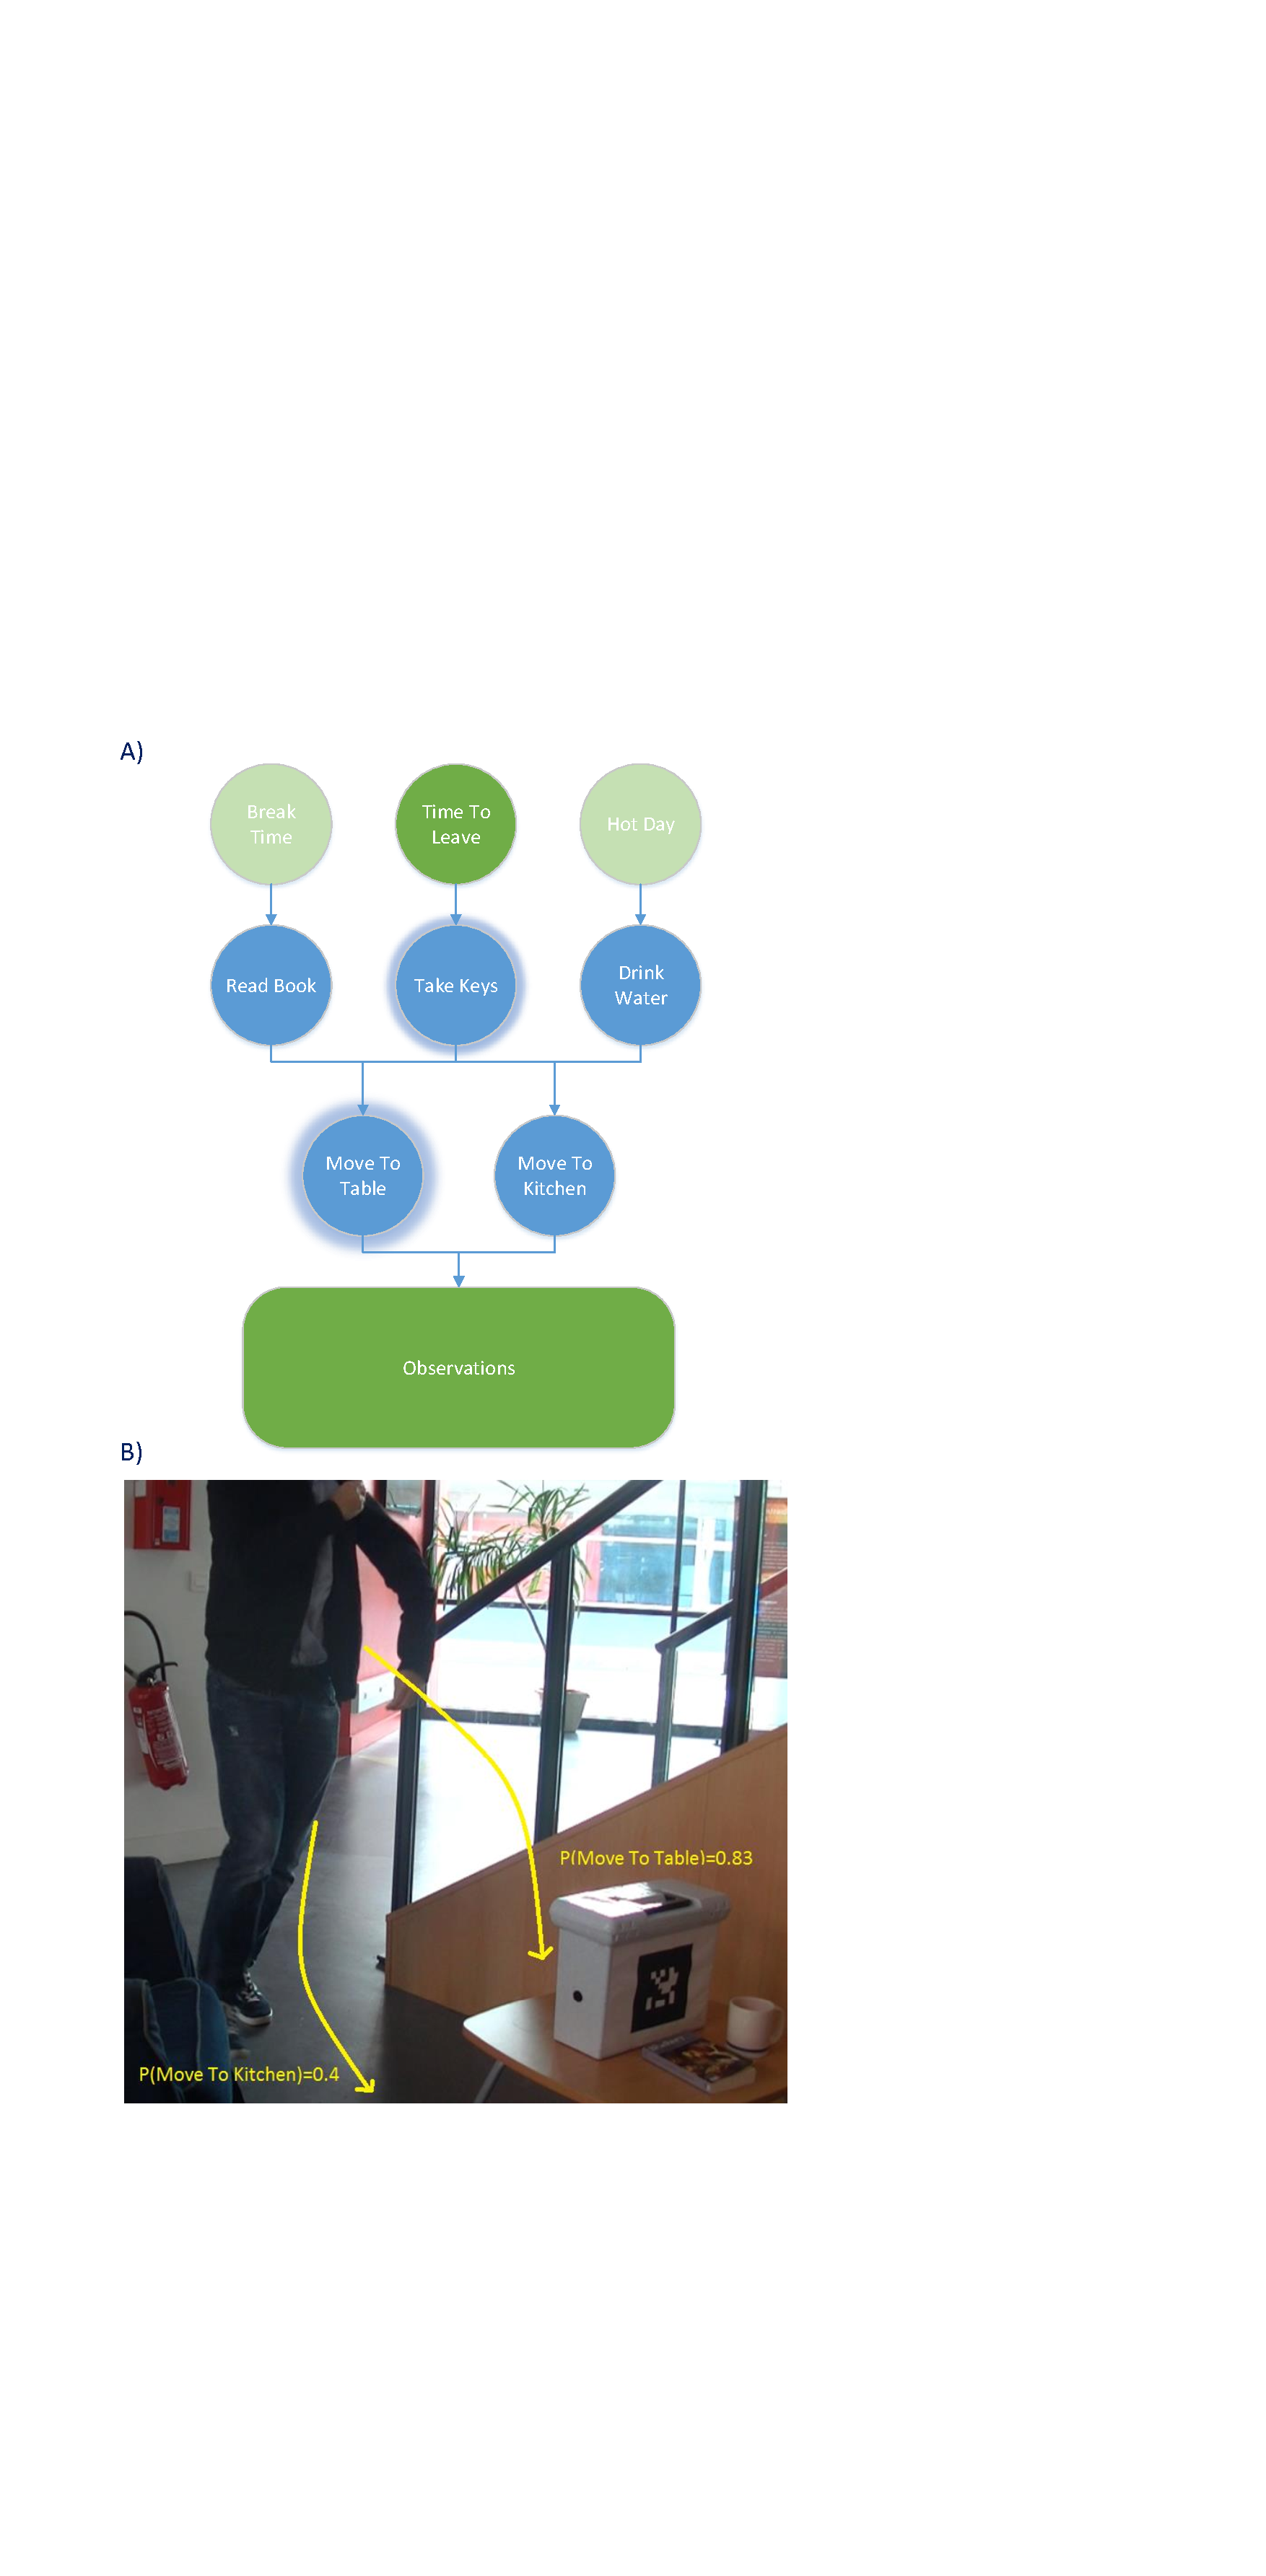
\includegraphics[trim={2cm 11cm 11cm 17cm},clip,scale=0.45]{img/observer/cookieScenario.pdf}
	\caption[Intention Graph]{A scene from our experiment. The yellow arrows show possible actions and their associated probabilities. The diagram represents the current IG. Green circles represent evidence nodes and blue circles other nodes. For the Context Nodes (top of the graph), we represented nodes with a false value as greyed out, and nodes with a true value as green. The most likely nodes in the graph are represented with a glowing effect. The observation nodes were compressed in a single block to simplify the diagram}
	\label{fig:intention-intention_graph}
\end{figure}

The following subsection will provide details on the IG, while section~\ref{sec:intention-example} will show an example of its use.

\subsection{From Contexts to Intentions}
We introduce a set of contexts in our domain. We consider as context any information that can be used to characterize and motivate an intention \citep{abowd1999towards}. We model a context  as a fact, which can assume different values and influences the probability of a user having a particular intention. For example, we imagine that a human is more likely to be cooking at dinner time, or to drink a hot mug of tea on a cold day.

Contextual nodes can directly influence one or more Intention nodes. In this work, we chose to learn these conditional dependencies from humans, as explained in section~\ref{sec:intention-experiments}.

\subsection{From Intentions to Actions}
\label{sec:intention-action_evaluation}
To understand how actions are linked to intentions the robot needs to answer the following question: what actions would a human take, in this situation, given his belief of the world, in order to achieve its intention?
Our idea is based on the principle of rationality \citep{Dennet1989}, which states that agents tend to choose the most efficient actions, taking into account their beliefs about the world, in order to achieve their desires.

In~\cite{Blakemore2001}, the authors explain that ``the attribution of intentions to actions might rely on simulating the observed action and mapping it into representations of our own intention". We represent this idea by providing the robot with a set of planning models. Each one of these planning models is related to an intention, and represents all the known plans to achieve its linked goal. In this way, we can estimate how much the current human actions are compatible with the plans related to an intention.

In our implementation, for each intention known by the robot, we will create an associated Markov Decision Process (MDP), to represent all the possible plans linked to this intention. After solving the set of MDPs we will use the calculated action value function \(Q(s,a)\), to create conditional dependencies between Intention and Action nodes in the IG. We define \(P(a|I_i=1)\), the probability that action $a$ will be performed if intention $I_i$ is true, as as:
\begin{equation}
 P(a|I_i=1)=\frac{Q_i(s,a)}{\sum_b(Q_i(s,b))}
\end{equation}
  where we normalize the value function $Q_i(s,a)$ for intention $i$ and action $a$ in the human's belief state $s$, over the value function $Q_i(s,b)$ calculated on all the monitored actions $b$. 

%   We can extend this calculation to the case where a generic number of intentions are true to compute the probabilities of action nodes: 
% \begin{equation}
%   P(a|I_1,I_2,...,I_m)=\frac{\sum_{i:I_i=1}Q_i(s,a)}{\sum_b\sum_{i:I_i=1}Q_i(s,b)}
% \end{equation}

The key idea in this problem is to use the human's belief state as input for the MDPs' value functions. In this way we are using perspective taking at a planning level, since the human action will be consistent with his intention in his own belief state but may be not optimal, irrelevant, or even dangerous in the real world (e.g. in case of wrong belief).

Our idea is similar to \cite{karami2010human}. In this work, the robot planning model is a POMDP, where the human intention is a hidden variable. The transition function for the human intention is computed starting from the action values obtained from a set of human MDPs, that simulate human policies related to different intentions. In this work, we used a BN for the inference process, instead of a POMDP. This allows us to include in a simple way more information in the inference process, such as context, and to separate the mechanisms used for inference and for the robot's actions. Also, we improve the recognition process by including the belief state of the human.

\subsection{From Actions to Observations}
Intentions will be inferred from human actions, so the robot needs to monitor their execution. For each Action Node we can define a different set of Observation Nodes, which depend on the specific actions. Typical examples are: the distance of the human's body from the action's $target$, its variation, the distance of the human's hand from the action's $target$, and its variation. The conditional dependencies of the Observation Nodes are precomputed.

\subsection{Intention and Action Inference}
\label{sec:intention-intention and action inference}
We assume, in this work, that at each moment a human can only execute a single action, and the robot will react only to his most likely intention. The most likely action and intention are inferred from the BN in the following way. We call $P(n)$ the inferred probability of a node $n$, $B(n)$ the set of brothers of $n$ (that is, nodes on the same layer), and $\delta_1$, $\delta_2$ two thresholds. The robot selects the most likely action and intention following these rules: 
\begin{itemize}
\item  \(P(n_i)>\delta_1\) 
\item  \(\forall b \in B(n_i): P(n_i)>P(b)+\delta_2\), where $n_i$ is the node associated to the interested intention or action.
\end{itemize}

To infer that an action has been performed, the robot uses an estimation of the action's probability and geometrical reasoning. For example, the robot infers that a human has taken a bottle if his hand is closer to it than a threshold $\sigma$  and the action's probability in the IG respect the previous rules. For another example, the robot infers that a human has mixed some ingredients in a bowl if his hand approaches the bowl and then leaves after some seconds, always taking into account the probability of the action in the IG.

When the robot infers that an action has been performed, it updates the world state with its $postconditions$, triggering an update on the beliefs of all present agents. The current human intention is recorded in the Database, and will be used by the Goal Management layer.

 \begin{figure}[ht!]
	\centering
	\includegraphics[scale=0.8, trim={0 4cm 0 0}]{img/observer/pick.pdf}
	\caption[Actions and world update]{The human picks an object and the robot updates accordingly the world state. The spheres surrounding objects show when the human's hand is considered to be near an object.}
	\label{fig:intention-pick}
\end{figure}

\subsection{Action Inference with Unknown Intentions}
In some situations, we are interested in inferring human actions without using information from intentions. One situation is when we the robot as a shared plan with a human. The MDPs used in our implementation are able to plan only for a single-agent, and can not be used to represent the shared plan. This could be a problem, because when agents act alone, they might execute different actions than when acting together. For example, if Greg and the robot are reordering a room together, Greg might give the robot a book, because in the shared plan the robot will put it in its place. If Greg is acting alone, he will need to place the book back by himself.  

In this situation, we will create an IG using only actions and observations. In this way, we can still infer which actions are executed, but we have to rely only on geometrical reasoning. Since we are using limited perception algorithms, we could easily encounter ambiguous situation, where, for example, the human moves his hand toward two close objects. In this situation, without using higher level information, the system could make mistakes, and infer that the wrong action has been performed.

We will discuss, in chapter~\ref{chapter:mamdp} about a possible multi-agent implementation to solve this issue.

\section{Proactive Behaviors}
\label{subsec:intention-proactive_behaviors}
Information about the most likely intention and action will be introduced in the Situation Assessment layer's Database, to be read by the Goal Management layer. Based on this information, the robot can execute two different proactive behaviors: correcting the belief state of the human, and proactively helping him to achieve his task.

\subsection{Correcting Belief State}
Having a wrong or incomplete belief on the world state can lead agents to execute non optimal, useless, or even dangerous actions. The robot needs to detect these situations in order to warn the human. For example Greg could search for his glasses in a wrong location if he does not know that they were moved, or could touch a hot object if he does not know its temperature.

 The robot assumes that it always holds a correct belief state. Our solution uses the expected action rewards introduced in \ref{sec:intention-action_evaluation}. The idea is comparing the expected reward for performing an action according to the human and the robot's belief states. To formalize: we compare the action values \(Q_m(s_h,a_h)\) and \(Q_m(s_r,a_h)\), where $m$ is the most likely intention,  $s_h$ and $s_r$ are the robot's and human's belief state, and $a_h$ is the most likely action. If these values are not equal the human expects a different outcome from its action than what should actually happen. 

We propose a simple solution, where the robot warns the human of the detected divergent belief for that action. For example, Bob wants to drink tea from a closed, opaque bottle, which the robot knows is empty (perhaps because another agent drank the last glass), while Bob does not. When he approaches the bottle, the robot detects that his most likely intention is to drink tea. 

The system calculates the expected rewards from taking the bottle in the two belief models and obtains different values. The system checks the facts related to the attributes associated to the target of the action (i.e. the bottle) in the two mental models, and extracts the differences.  Using this information, the robot corrects the divergent belief, informing the human that the bottle is now empty. 

If there is no difference in the belief models, it means that the divergent belief is actually related to a future action that the human is expected to execute. For example, let us imagine a scenario where Greg is trying to prepare a dish, requiring pasta and tomatoes. Let us imagine that Greg does not know that there are no more tomatoes, and moves to take the pasta. Using Greg's belief model, there will be a certain reward to take the pasta, since it is a necessary step to prepare the dish. In the robot's belief model, the reward will be zero (assuming that he correctly inferred the intention of Greg to prepare pasta with tomato sauce), because there are no more tomatoes. While there are is no divergent belief on attributes related to the pasta, it would be useful if the robot would inform Greg that there are no more tomatoes.

A solution is extracting an horizon of future actions from the MDP related to the \textit{prepare pasta with tomato sauce} intention. Our system can do this by simulating an update on the MDP, considering as starting state the current human belief model, choosing as actions from the agent's policy computed when solving the model, and taking as next states the most likely effects of the actions. We can repeat the reasoning on the targets of each action in this horizon, in order to find a divergent belief. 

If we can still not find a divergent belief, the robot can only inform a human that there might be a problem to achieve its goal, but it is not able to identify it.

% In our system, the Goal Management layer will detect these situations, by reading the Database, and choose a \textit{warn agent} goal (as will be explained in chapter \ref{chapter:goal_management}).

In a real scenarios, the human might have several divergent beliefs at the same time. While the robot could inform the human as soon as it detects a divergent belief, it would risk overloading him with unneeded information. For example, Greg might not know that his wife drank a mug of coffee or moved the remote control to the table, but maybe he will not need these information in the near future. We chose, with this approach, to give information about a divergent belief only when it risks impacting the actions of a human.

\subsubsection{Performing a part of the plan}
There are situations in which the robot should help the human achieve its goal by physically acting. The Goal Management layer will consider new inferred intentions as possible goals for the robot, and will communicate with the Plan Management layer to achieve them, as explained in chapters~\ref{chapter:plan_management} and~\ref{chapter:plan_execution}. 

\section{Intention Graph Example}
\label{sec:intention-example}

\subsection{Scenario}
We will now show an example of use of an IG. We start by defining a scenario with a human, Greg, and two possible intentions: drinking water and reordering a table, by moving all the objects on top of it to the kitchen. We set three different locations: a \textit{table}, a \textit{shelf}, and a \textit{kitchen}. We consider two objects: a \textit{glass} and a \textit{bottle}. Both these objects can contain water, but the \textit{bottle} is opaque and Greg can not observe if there is water or not in it. We simplify the situation by imagining that the bottle is already open. Of course, this scenario is not realistic and is chosen just to illustrate the IG. In a real situation Greg would notice that the bottle is empty when taking it, because it would be too light, or by looking through its hole.

At the start of the scenario, Greg is at the \textit{shelf}, the \textit{bottle} and \textit{glass} are on the \textit{table}, and the they are both empty.  We set a situation of divergent belief, where Greg does not know that the bottle is empty, but the robot has this information. 

We introduce two predicates: \textit{isAt}, that represented the location of an entity, and can assume the values \textit{TABLE}, \textit{SHELF}, and \textit{KITCHEN}; and \textit{capacity}, which indicates if an object contains water, and can assume the values \textit{0}, and \textit{1}. 

The belief models of Greg and of the robot are shown in table~\ref{table:intention-ig_bm}, while the set up for this scenario is shown in figure~\ref{fig:intention-ig_scenario}.

 \begin{table}[h!]
\centering
\scriptsize
\renewcommand{\arraystretch}{1.3}
\begin{tabular}{|c|c|}
\hline
Robot & Human \\ \hline \hline
GLASS isAt TABLE  & GLASS isAt TABLE \\ \hline
BOTTLE isAt TABLE & BOTTLE isAt TABLE \\ \hline
GLASS capacity 0  & GLASS capacity 0  \\ \hline
BOTTLE capacity 0 & BOTTLE capacity 1 \\ 
\hline
\end{tabular}
\caption[Belief models in the IG scenario]{Belief models for Greg and for the robot in the IG example scenario. There is a divergent belief situation, where Greg does not know that the bottle is currently empty, represented by the fact \textit{BOTTLE capacity VALUE} }
 \label{table:intention-ig_bm}    
\end{table}



 \begin{figure}[ht!]
	% \centering
	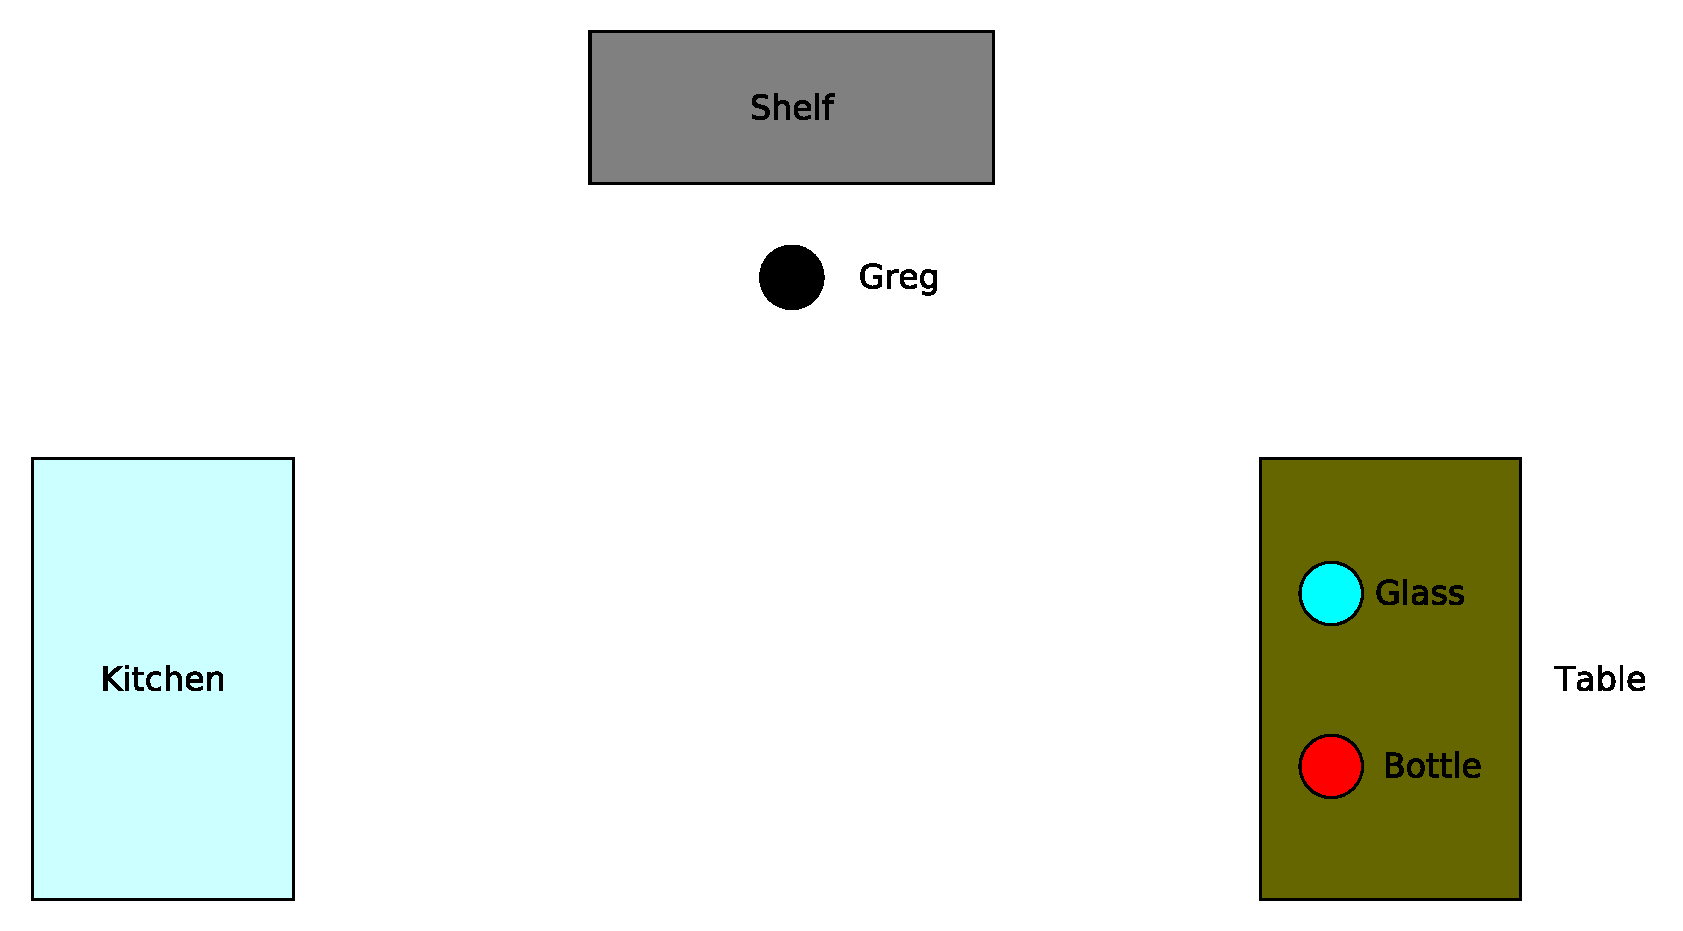
\includegraphics[scale=0.5]{img/observer/ig_scenario.pdf}
	\caption[IG Example Scenario]{The image shows the set-up for the IG example scenario. The locations are represented as different rectangles. Greg is represented as a black circle. The glass and bottle are represented, respectively, by a blue circle and a red circle.}
	\label{fig:intention-ig_scenario}
\end{figure}

We introduce two contexts in the scenario: \textit{HotDay}, representing the fact that the day is particularly warm, and \textit{AlreadyDrank}, representing the fact that the human has recently drank water.

We introduce this possible set of actions in the scenario: taking the bottle, taking the glass, filling the glass using the bottle, drinking from the glass, moving to the kitchen, moving to the table, placing the objects in different locations. We simplify this set to only include the actions relevant to this example, and so we do not include the possibilities for Greg to refill the bottle with water. Also, we consider that Greg can only hold a single object at a moment. 

\subsection{Building the Intention Graph}
We build a starting IG with the following nodes:
\begin{itemize}
	\item Context Nodes: \textit{HotDay}, \textit{AlreadyDrank}.
	\item Intention Nodes: \textit{DrinkWater}, \textit{ReorderTable}.
	\item Action Nodes: \textit{MoveTable}, \textit{MoveKitchen}. These two actions are introduced in the IG because they are the only ones whose $preconditions$ are currently satisfied, since Greg can move in any location where he is not at the moment.
	\item Observation Nodes: \textit{BodyDistanceTable}, \textit{TowardTable}, \textit{BodyDistanceKitchen}, \textit{TowardKitchen}. The \textit{BodyDistance} nodes represent the distance between Greg and an object, and can assume the values \textit{close}, \textit{medium}, \textit{far}, \textit{out of range}. The \textit{Toward} nodes are \textit{true} if the distance between \textit{Greg} and the object is decreasing, and false otherwise.
\end{itemize}


In this scenario, we precompute the probability table of the causal links between Context Nodes and Intention Nodes, and between Action Nodes and Observaton Nodes. We set a causal link between \textit{HotDay} and \textit{DrinkWater}, and one between \textit{AlreadyDrank} and \textit{ReorderTable}. In both cases, we use the following probability table:

 \begin{table}[h!]
\centering
\begin{tabular}{|c|c|c|}
\hline
Context & \multicolumn{2}{|c|}{Intention} \\ \hline \hline
& 0 & 1 \\ \hline
0  & 0.6 & 0.4 \\ \hline
1 & 0.4 & 0.6 \\ \hline
\end{tabular}
\caption[Belief models in the IG scenario]{Conditioned probabilities of the Intention Nodes in the IG example scenario.}
 \label{table:intention-ig_intention}    
\end{table}

We consider as slightly more likely that Greg wants to drink water in a Hot Day, and that he wants to reorder the table if he drank recently.

We set a causal link between each action and its observation nodes. For example, \textit{MoveTable} will have a causal link with \textit{BodyDistanceTable} and \textit{TowardTable}. In both actions, we use the following probability tables:

 \begin{table}[h!]
\centering
\begin{tabular}{|c|c|c|}
\hline
Action & \multicolumn{2}{|c|}{Toward} \\ \hline \hline
& 0 & 1 \\ \hline
0  & 0.8 & 0.2 \\ \hline
1 & 0.2 & 0.8 \\  \hline
\end{tabular}
\caption[Belief models in the IG scenario]{Conditioned probabilities of the Toward Nodes in the IG example scenario.}
 \label{table:intention-ig_toward}    
\end{table}

 \begin{table}[h!]
\centering
\begin{tabular}{|c|c|c|c|c|}
\hline
Action & \multicolumn{4}{|c|}{Distance} \\ \hline \hline
& Close & Medium & Far & Out of Range \\ \hline
0  & 0.16 & 0.2 & 0.25 & 0.39 \\ \hline
1 & 0.39 & 0.25 & 0.2 & 0.16 \\ \hline
\end{tabular}
\caption[Belief models in the IG scenario]{Conditioned probabilities of the Distance Nodes in the IG example scenario.}
 \label{table:intention-ig_distance}    
\end{table}

If Greg is executing an action, it  more likely that he is moving toward the action's $target$. For example, the \textit{MoveTable} action is more likely the closer Greg is to the table and if the distance to it is decreasing.

\subsection{Building the Human MDPs}
To set the conditioned probabilities between Intention and Action Nodes, we created two different MDPs, each related to one of the intentions. We will now show the state space $S$, action set $A$ and reward function $R$  of the two MDPs. We do not include the transition function of the model as it is extensive and does not help understanding this example.

\begin{itemize}
\item DrinkWater:
\begin{itemize}
\item $S$: $\{agent\_isAt, glass\_isAt, bottle\_isAt, bottle\_capacity, glass\_capacity\}$.
\item $A$: $\{agent\_move\_table, agent\_move\_kitchen, agent\_move\_shelf, agent\_take\_bottle, \\ 
agent\_take\_glass, 
agent\_fill\_glass\_bottle, agent\_drink\_glass, agent\_place\_bottle\_table, \\ agent\_place\_bottle\_kitchen, agent\_place\_bottle\_shelf, agent\_place\_glass\_table, \\ agent\_place\_glass\_kitchen, agent\_place\_glass\_shelf\}$.
\item $R(s,a)=1000 \quad \text{if} \\
glass\_isAt==agent\_isAt \; \text{AND} \; glass\_capacity==1  \; \text{AND} \; a==agent\_drink\_glass$.
\end{itemize}


\item ReorderTable:
\begin{itemize}
\item $S$: $\{agent\_isAt, glass\_isAt, bottle\_isAt\}$.
\item $A$: $\{agent\_move\_table, agent\_move\_kitchen, agent\_move\_shelf, agent\_take\_bottle,\\ agent\_take\_glass, 
agent\_place\_glass\_kitchen, agent\_place\_bottle\_kitchen\}$.
\item $R(s,a)=1000 \quad \text{if} \\
(glass\_isAt==kitchen \; \text{AND} \; bottle\_isAt==human \; \text{AND} \; a==human\_place\_bottle\_kitchen)  \\
 \text{OR} \\
 (glass\_isAt==human \; \text{AND} \; bottle\_isAt==kitchen \; \text{AND} \; a==human\_place\_glass\_kitchen)$.
\end{itemize}
\end{itemize}

After solving these MDPs we used their action value functions to compute the conditioned probabilities for the Action Nodes, as shown in section~\ref{sec:intention-action_evaluation}.

\subsection{Simulated Run}
We will now show a simulated run of this scenario in three steps. This run was created by introducing a stream of observations in the system, including the actions that Greg will perform. We consider that Greg's intention in this example is \textit{Drink Water}. We will conduct three different tests for each step:
\begin{itemize}
	\item Test 1. We create the IG using the human's mental belief state to compute the causal links between Action and Intention nodes. We do not use context to help disambiguate the intentions.
	\item Test 2. We add contextual information to Test 1, setting \textit{HotDay} to \textit{true} and \textit{RecentlyDrank} to \textit{false}.
	\item Test 3. We do not use contextual information and use the robot's mental belief state to compute the causal links between Action and Intention nodes. This means that the robot will evaluate Greg's action by considering that he knows that the bottle is currently empty (even though he does not know).
\end{itemize}

We will now describe and discuss these stages:
\begin{itemize}
	\item Greg is approaching the \textit{table}, as shown in figure ~\ref{fig:intention-ig_exp1}. The observations are updated correspondingly, and the probabilities of the actions are computed. The action \textit{MoveTable} has the highest probability. 
		\begin{itemize}
			\item Test 1. At this stage, the system is not able to infer the correct intention. Greg could be going to the \textit{table} to take the objects and bring them to the \textit{kitchen} or to drink water. The probability of the two intentions is both 0.50.
			\item Test 2. By using context, the system is already able to infer the correct intention. The probability of \textit{DrinkWater} becomes 0.69, and that of \textit{ReorderTable} 0.3. The robot could already fire a proactive behavior to inform Greg that the \textit{bottle} is, in fact, empty.
			\item Test 3. Without context, the system thinks that Greg is trying to reorder the table, since it is not possible to drink water because the \textit{bottle} is empty. The system would infer a wrong intention.
		\end{itemize}
	\item Greg has arrived to the \textit{table}, as shown in figure~\ref{fig:intention-ig_exp2}. The $postconditions$ of the action are added to the mental models of the robot and of Greg, changing Greg's location. The system creates a new IG, setting as actions those whose $preconditions$ are now satisfied: \textit{MoveKitchen}, \textit{MoveShelf}, \textit{TakeGlass}, and \textit{TakeBottle}. At this point, Greg's hand moves toward the \textit{bottle}, and the observations nodes are set appropriately.
		\begin{itemize}
			\item Test 1. The system is still not able to disambiguate between the two intentions. Greg could be taking the  \textit{bottle} to fill the \textit{glass} or to bring it to the \textit{kitchen}.
			\item Test 2. In this case, the context is still providing the missing information to understand that Greg wants to drink water.
			\item Test 3. In this case, since it is not possible to drink water in the robot's mental belief, the system is still inferring the wrong intention.
		\end{itemize} 
	\item Greg has taken the \textit{bottle}, and is now bringing it to the \textit{glass}, as shown in figure~\ref{fig:intention-ig_exp3}. A new IG is created, containing the actions that are now executable: \textit{MoveKitchen}, \textit{MoveShelf}, \textit{PlaceBottleTable}, and \textit{FillGlass}. In test 3, the IG created would not contain the action to fill the glass with water, since it is not executable in the robot's mental belief model, where the \textit{bottle} is empty.
		\begin{itemize}
			\item Test 1. At this point, the system has enough information to understand that Greg's intention is \textit{DrinkWater}, which assumes a probability of 0.90. The system can now fire a proactive behavior, with the robot informing Greg of the divergent belief. Even tought the action \textit{PlaceBottleTable} and \textit{FillGlass} could be ambiguous from a geometric point of view (since, in both cases, the arm of the human will approach the table), the system could infer that the action performed was \textit{FillGlass} since it is more \textit{useful} in the current situation and with the considered intentions.
			\item Test 2. Context confirms this intention, bringing the probability to 0.99.
			\item Test 3. In this case, Greg's movement would not be understood, since in the robot's mental belief model it is not possible to fill the glass with water. Greg's action would actually be inferred as \textit{PlaceBottleTable}, which has no use for any intention.
		\end{itemize}
\end{itemize}

 \begin{figure}[ht!]
	\centering
	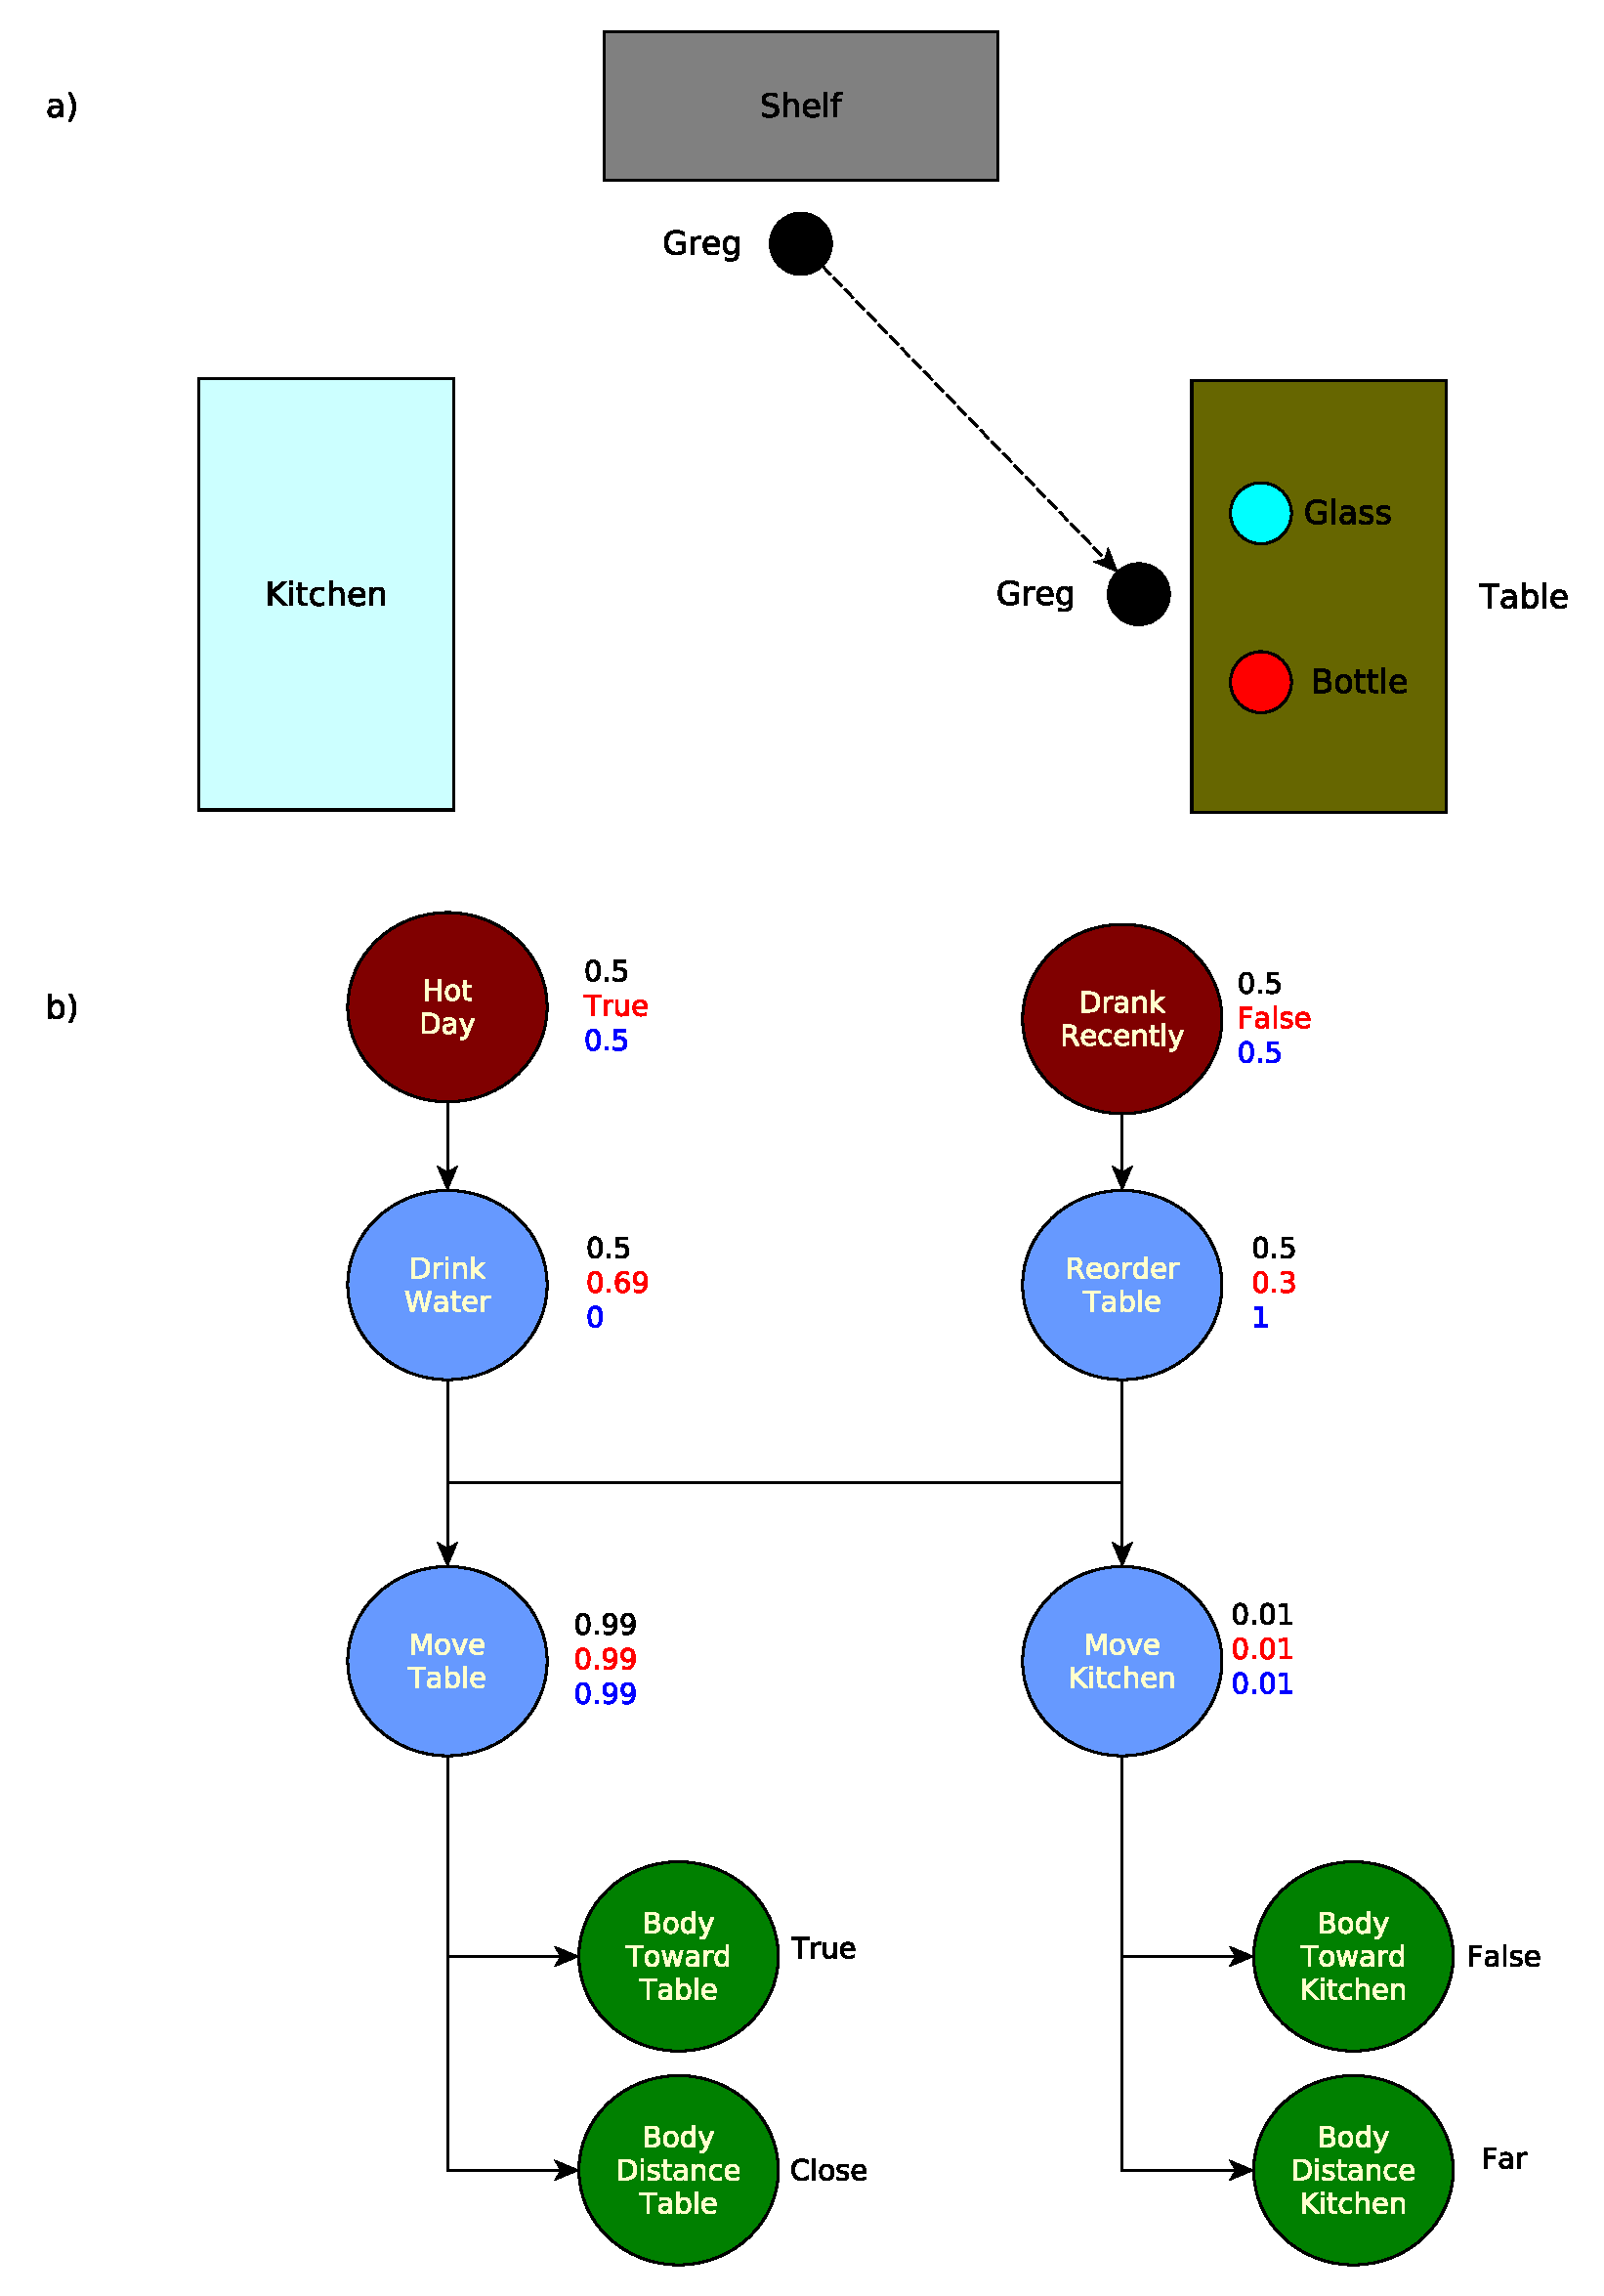
\includegraphics[scale=0.4]{img/observer/ig_exp1.pdf}
	\caption[IG Example 1]{a) Greg, represented as a black circle, is approaching the table. The two black circles correspond to his starting and ending location, with the dotted arrow showing the direction of his movement. b) The corresponding IG graph. Nodes are represented as circles and causal links as arrows. Intention and Action nodes are represented as blue. Observation nodes are represented as green to show that we consider them as evidence, fixing their values. Context nodes are represented in yellow to mean that in the first and third test they are treated as standard nodes, and in the second as evidence.
 	 For each node we show the probability that its value is true or its current value, if it is treated as evidence. We show three different values for each node: the black one shows the value if we compute the probability by using the human's mental belief (test 1), the red if we use the human's mental belief and treat context nodes as evidence (test 2), and the blue if we do not use context and use the robot's mental belief for the computation (test 3). Test 1 shows that at this point the system is not able to disambiguate between the two intention, which have a value of 0.50. Test 2 shows that context would help the robot to infer correctly the intention. Test 3 shows that by not using the human's mental belief the robot would discard the drink water intention, considering it not achievable.}
	\label{fig:intention-ig_exp1}
\end{figure}

\clearpage

\hfill
 \begin{figure}[ht!]
	\centering
	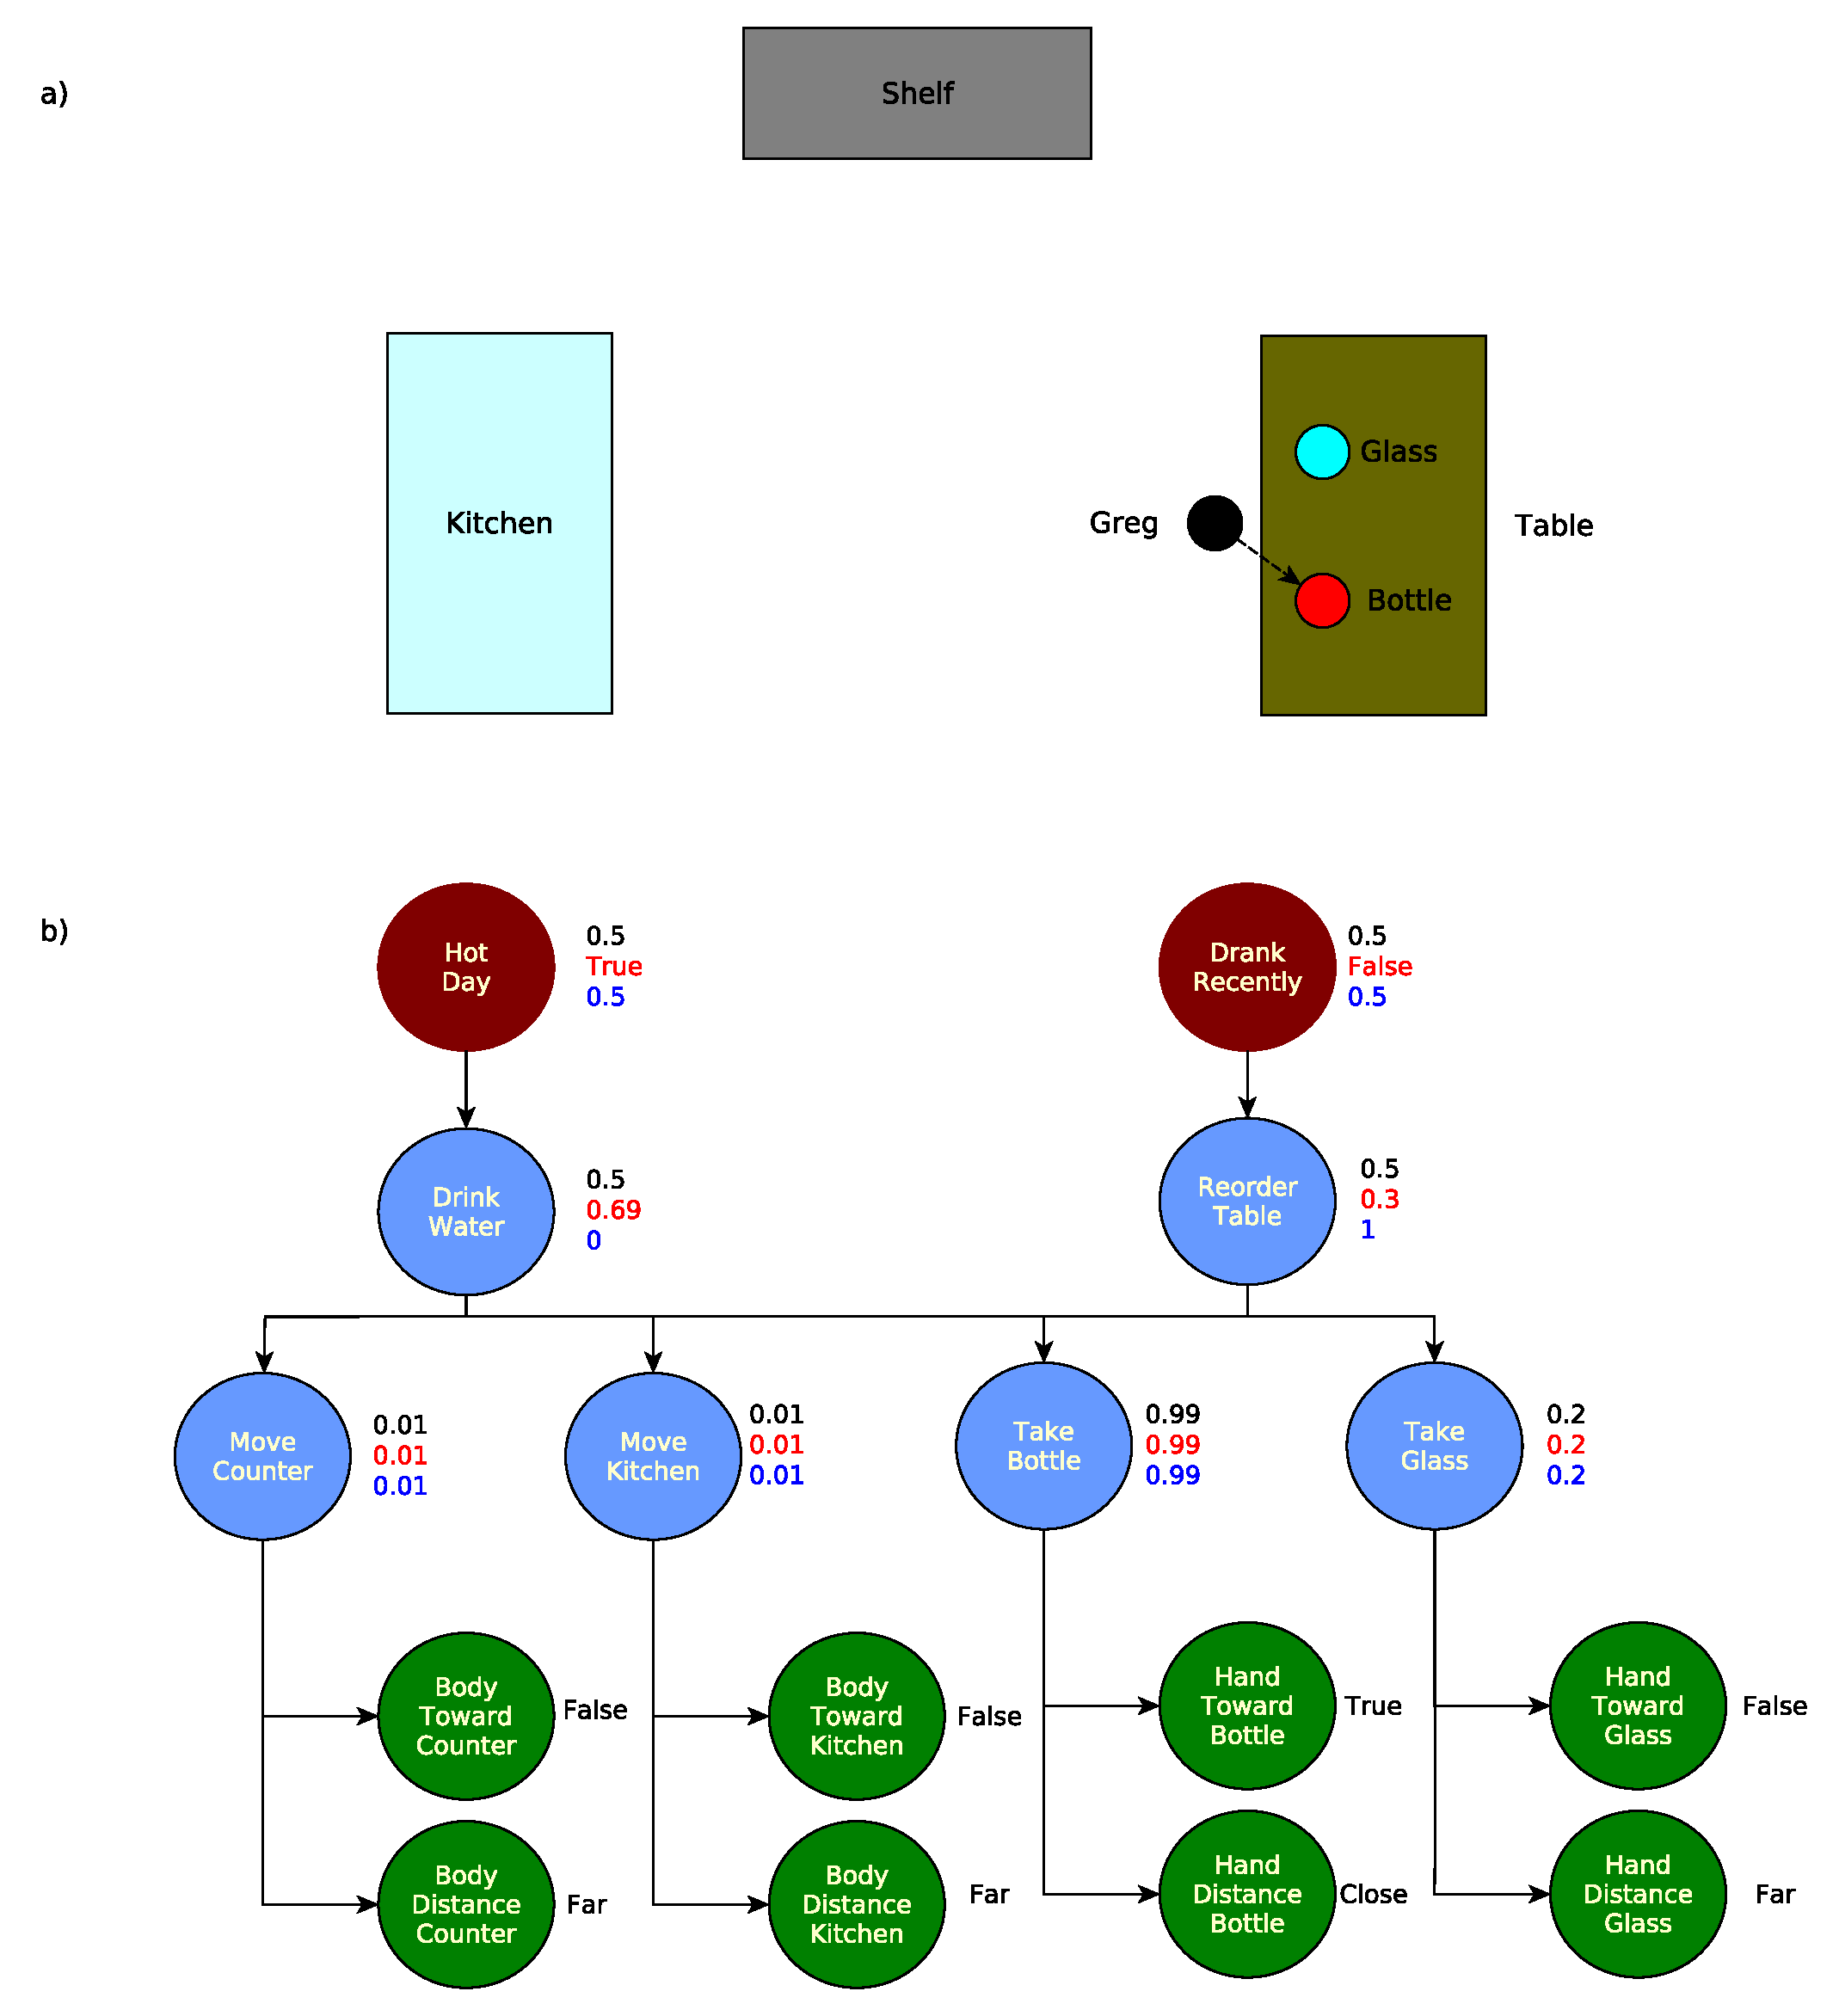
\includegraphics[scale=0.4]{img/observer/ig_exp2.pdf}
	\caption[IG Example 2]{a) Greg's hand is approaching the bottle. b) The corresponding IG graph. As before, test 1 is shown in black, test 2 in red, and test 3 in blue. The results of 
	the test are very similar to the previous time step, shown in figure~\ref{fig:intention-ig_exp1}.}
	\label{fig:intention-ig_exp2}
\end{figure}

\clearpage
 \begin{figure}[ht!]
	\centering
	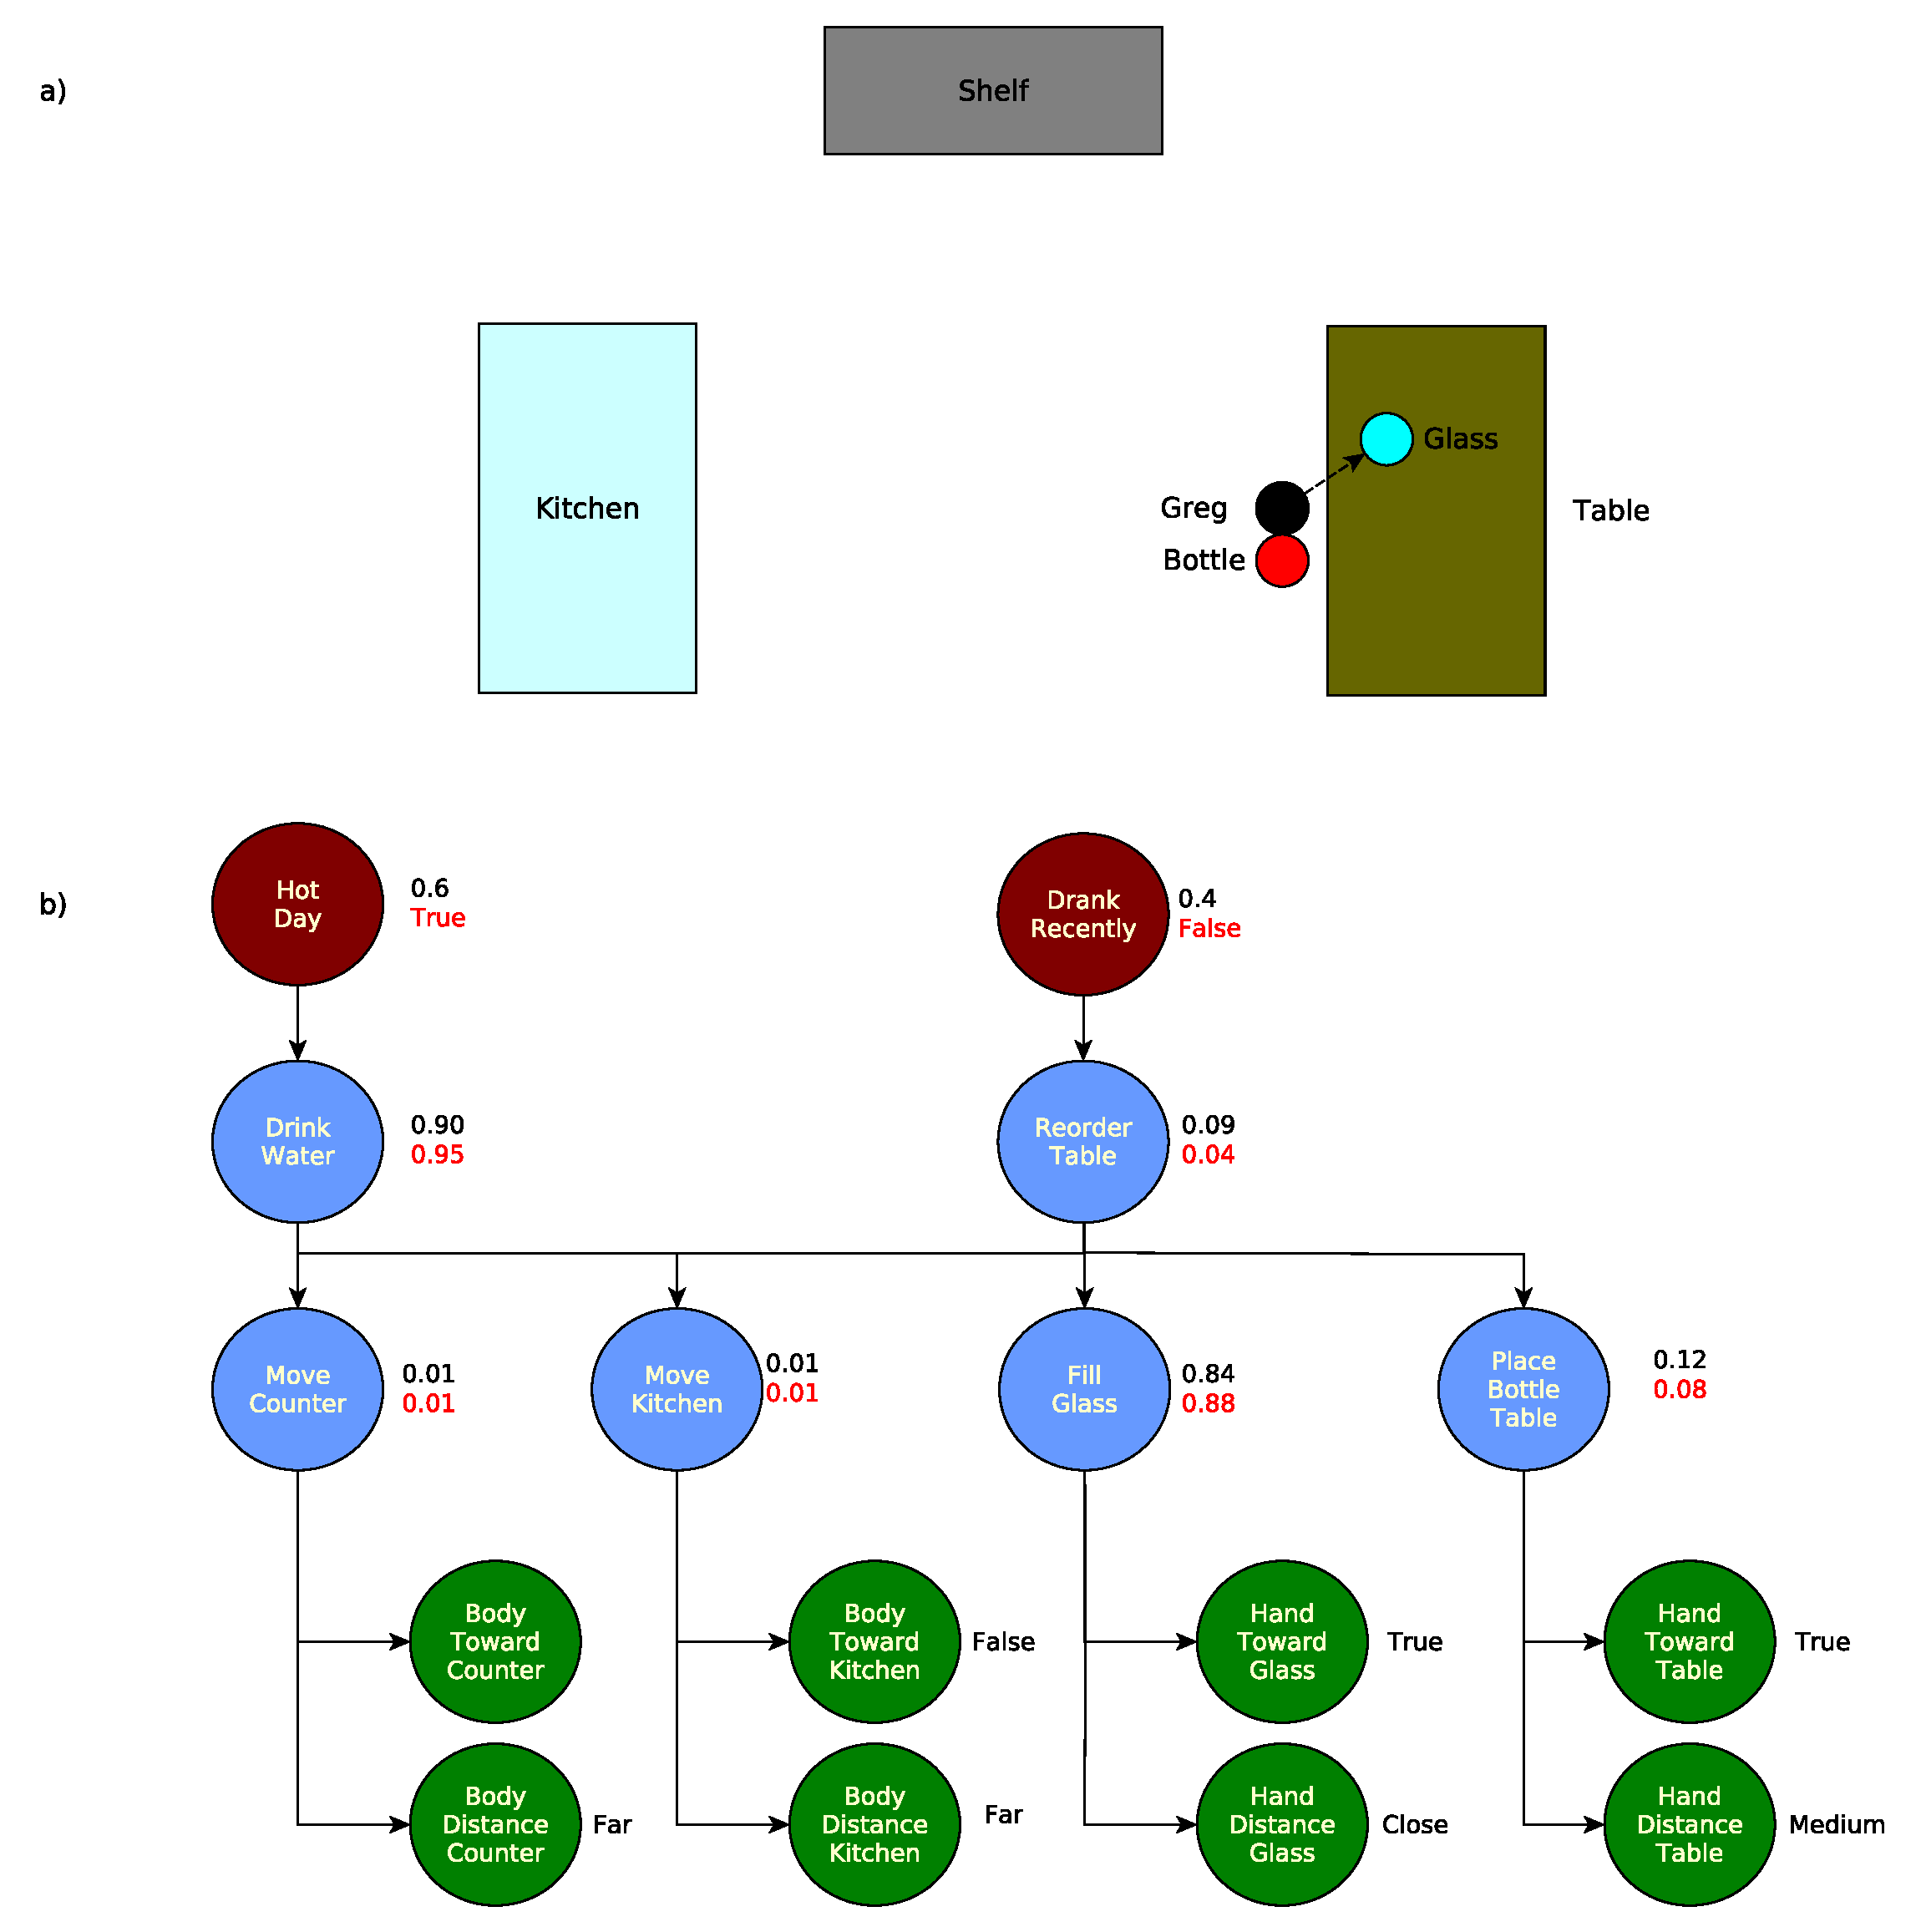
\includegraphics[scale=0.4]{img/observer/ig_exp3.pdf}
	\caption[IG Example 3]{a) Greg has taken the bottle, shown by placing the red circle and black circle close. His hand, with the bottle, is now approaching the glass b) The corresponding IG graph. As before, test 1 is shown in black and test 2 in red. Test 3 is not shown since the fill glass action would not be executable in the robot's mental belief model, and so the corresponding IG would be different. In test 1 the system has now sufficient information to infer the corrent intention, which has a value of 0.98. Test 2 confirms this choice.}
	\label{fig:intention-ig_exp3}
\end{figure}
\clearpage

\section{Discussion}

This component is able to estimate the likelihood of a human's intention by combining BNs, MDPs, geometrical reasoning, and the capacity to model human's beliefs. Contextual information can further help to disambiguate the inference process. 

Another advantage of our approach is its good scalability. Computing the probabilities in a BN can be done using efficient and well know algorithms, which scale well with the size of the network, meaning that the IG is able to accomodate the addition of new actions, observations and contexts. 

Adding a new intention means creating and solving another MDP. Since this process is done offline this would not impact the run of the system. When computing the conditional probabilities of the action nodes, the system uses the action value function of the MDPs, which is stored in memory and can be directly accessed.
 
\chapter{Results and Experiments} % Main chapter title

\label{chapter:observer_results} % Change X to a consecutive number; for referencing this chapter elsewhere, use \ref{ChapterX}

\lhead{Chapter 4. \emph{Results and Experiments}} % Change X to a consecutive number; this is for the header on each page - perhaps a shortened title

This chapter presents an experiment used to evaluate the intention recognition capacity of our system. Section~\ref{sec:observer_experiment-case_study} introduces our case study, where we decided to compare the prediction of our system with those of humans. Section~\ref{sec:observer_experiment-experiment} explains how the experiment was actually conducted. We show and discuss our results in section~\ref{sec:observer_experiment-discussion}.


\section{Case Study}
\label{sec:observer_experiment-case_study}
\subsection{Study Description}

Evaluating the capacity of the system to estimate human intentions is not easy, since intentions are not directly observable. A possible solution, as shown in~\cite{baker2014modeling}, is comparing the estimation of human intentions, performed by other humans, with the predictions of our system. In order to perform this comparison we created a user study where we showed participants several videos, asking them to estimate the likelihood of a set of intentions  for each video, and collected their results. The same tests were simulated on the system, streaming as input a sequence of observations  corresponding to the actions shown in the video (e.g. if the video shows a human approaching the table, we will stream to the system a trajectory of coordinates that leads to the table position). All of the test videos ended in a situation of ambiguity. For example, in one test we showed a human approaching a table with different objects, and stopped the video before users could see which object the human wanted to take. Some videos include more information than others, like comments by humans or situations that help to disambiguate the intention. 

We have performed an equivalence test, comparing users' intentions predictions with those of the system, following the two one-sided tests (TOST) approach. We choose as a threshold for equivalence the standard deviation $\sigma$ of the users' answers. The idea behind this choice is that, if the system's answers are closer than a standard deviation to the average human answers, its predictions are comparable to an average human answer from our user group. 

We defined our hypothesis as follow: 
\begin{itemize}
\item $H_0$: $\mu_{hi}-\mu_{si}\leq-\sigma_{hi}$ \; \text{OR} \; $\mu_{hi}-\mu_{si}\geq\sigma_{hi}$ 
\item $H_A$: $-\sigma_{hi}<\mu_{hi}-\mu_{si}<\sigma_{hi}$  
\end{itemize}
where $\mu_{hi}$ and $\mu_{si}$ are the human average and the system's answer for test $i$, $\sigma_{hi}$ is the variance of the human answers for test $i$.

We have performed tests to evaluate: a) prediction in absence of clues, b) prediction in the presence of contextual clues, c) prediction in the presence of belief state clues.

We have built a household environment with a fixed set of furniture: a \textit{Kitchen Shelf}, a \textit{Table}, a \textit{Sofa}, and a \textit{Chair}. In this environment, we have created two scenarios, composed by several tests, with two agents, \textit{Max} and \textit{Bob}, performing different actions. Each scenario contained a set of objects, and a constrained set of intentions. For the tests related to belief states, we start by showing the users a specific sequence of events, allowing them to build a mental model of the agents. A corresponding simulated sequence will be streamed to the system for this test.
We will describe in details the two scenarios and the relative tests.

\subsection{Cookie Scenario}
\begin{itemize}
\item Objects: a \textit{Cookie Box}, a \textit{Mug}, and a \textit{Bottle of Water} were placed on the \textit{Table}, close to each other. A pack of \textit{Cookies} was placed on the \textit{Kitchen Shelf}. The \textit{Cookie Box} could contain, or not, \textit{Cookies}.
\item Intentions: \textit{Eating a Cookie}, \textit{Drinking Water}, \textit{Reading the Book}.
\item Tests:
\begin{itemize}
	\item \textit{No Clues}: \textit{Max} approaches the \textit{Table}.
    \item \textit{Contextual Clues}: \textit{Max} approaches the \textit{Table} commenting on the warmth of the day.
	\item \textit{Divergent Belief No Cookies}: \textit{Max} approaches the \textit{Table}.
	\item \textit{Divergent Belief Cookies}: \textit{Bob} approaches the \textit{Table}.
\end{itemize}
\item  \textit{Divergent Belief Event}:  \textit{Max} and \textit{Bob} are chatting on the \textit{Sofa}. Max eats the last \textit{Cookie} from the \textit{Cookie Box} before closing it and leaving. While \textit{Max} is away, \textit{Bob} takes \textit{Cookies} from the \textit{Kitchen Shelf}, fills the \textit{Cookie Box} with them, and closes it, before leaving.
\end{itemize}

The \textit{Divergent Belief Event} was shown to the users (and its simulation streamed to the system) between the \textit{Contextual Clues} and the \textit{Divergent Belief No Cookiies} events. 


We have deliberately included an intention, \textit{Reading the Book}, without placing a book in the visible environment, introducing a confusing element in the scenario. This scenario can be seen in figure~\ref{fig:observer_experiments-cookie}.


 \begin{figure}[ht!]
	\centering
	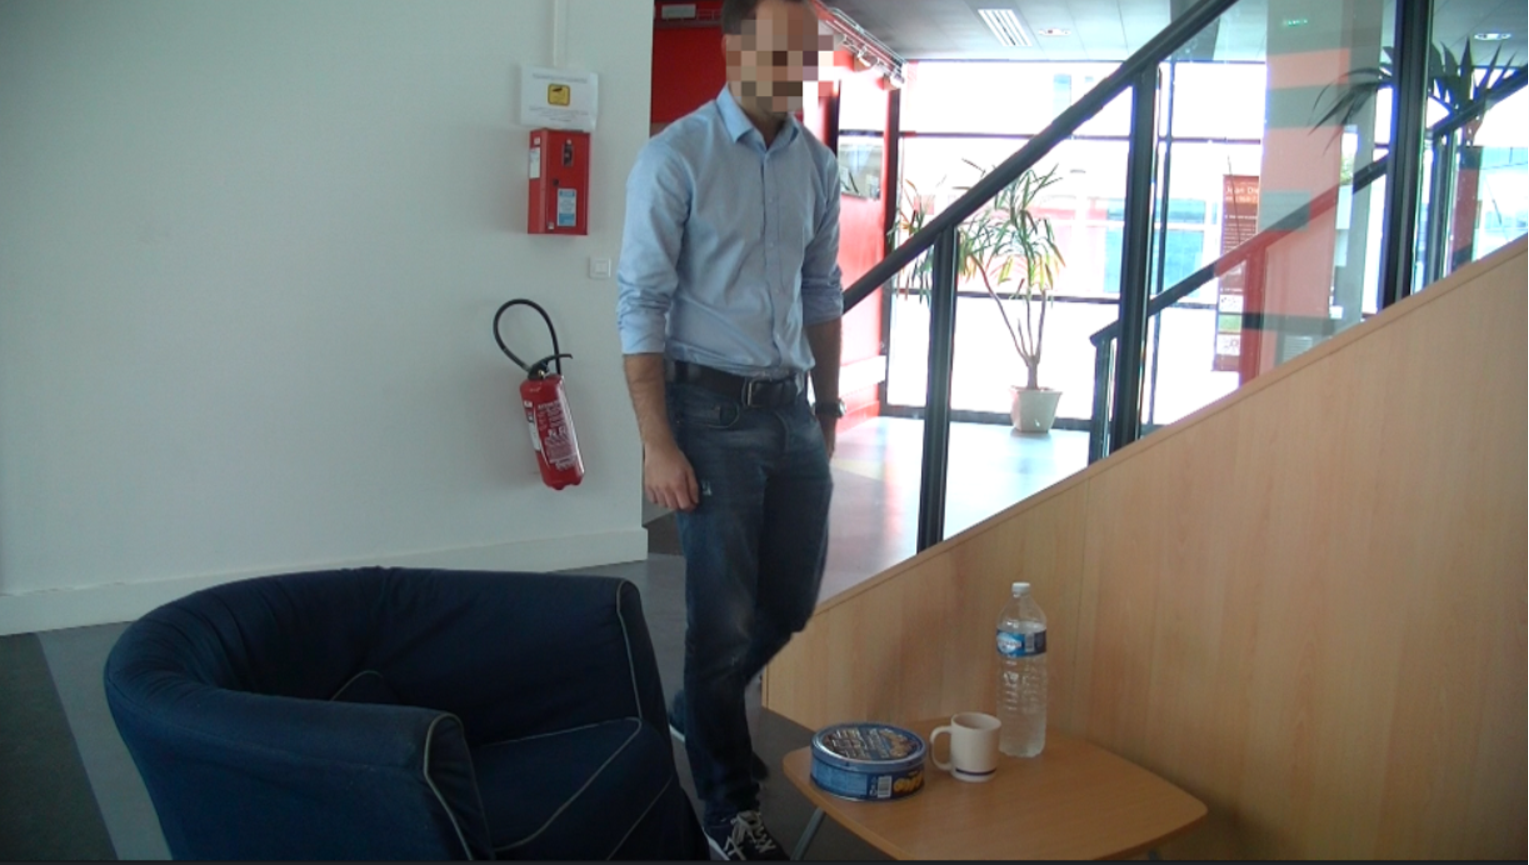
\includegraphics[scale=0.5]{img/observer/cookie1-blur.pdf}
	\caption{The cookie intention scenario}
	\label{fig:observer_experiments-cookie}
\end{figure}


\subsection{Keys Scenario}
\begin{itemize}
\item Objects: a \textit{Box} was placed on the \textit{Table}, that partially occluded the sight of people approaching. A \textit{Book} and a \textit{Mug} where placed behind the \textit{Box}, so that they could be seen from the sofa but not from approaching people.
\item Intentions: \textit{Taking the Mug}, \textit{Taking the Keys}, \textit{Reading the Book}.
\item Tests and Events:
\begin{itemize}
\item \textit{No Clues}: \textit{Max} approaches the \textit{Table}.
\item\textit{Contextual Clues}: \textit{Max} approaches the \textit{Table} in a hurry, while putting on a coat.
\item \textit{Divergent Belief Max}: \textit{Max} approaches the \textit{Table} in a hurry, while putting on a coat.
\end{itemize}
\item \textit{Divergent Belief Event}: \textit{Max} is sitting on the \textit{Table}, drinking from the \textit{Mug}, while having the \textit{Keys} in his hands. His phone rings, so he drops the \textit{Keys} and the \textit{Mug} on the \textit{Table}, behind the \textit{Box}, and leaves the room. While \textit{Max} is away, \textit{Bob} comes and sits on the \textit{Sofa}, reading a \textit{Book}. When he sees the \textit{Keys}, he takes them, places the \textit{Book} on the \textit{Table}, and leaves.
\end{itemize}

The \textit{Divergent Belief Event} was shown to the users (and its simulation streamed to the system) between \textit{Contextual Clues} and the \textit{Divegent Belief Max} events. This scenario can be seen in figure~\ref{fig:observer_experiments-keys}.

 \begin{figure}[ht!]
	\centering
	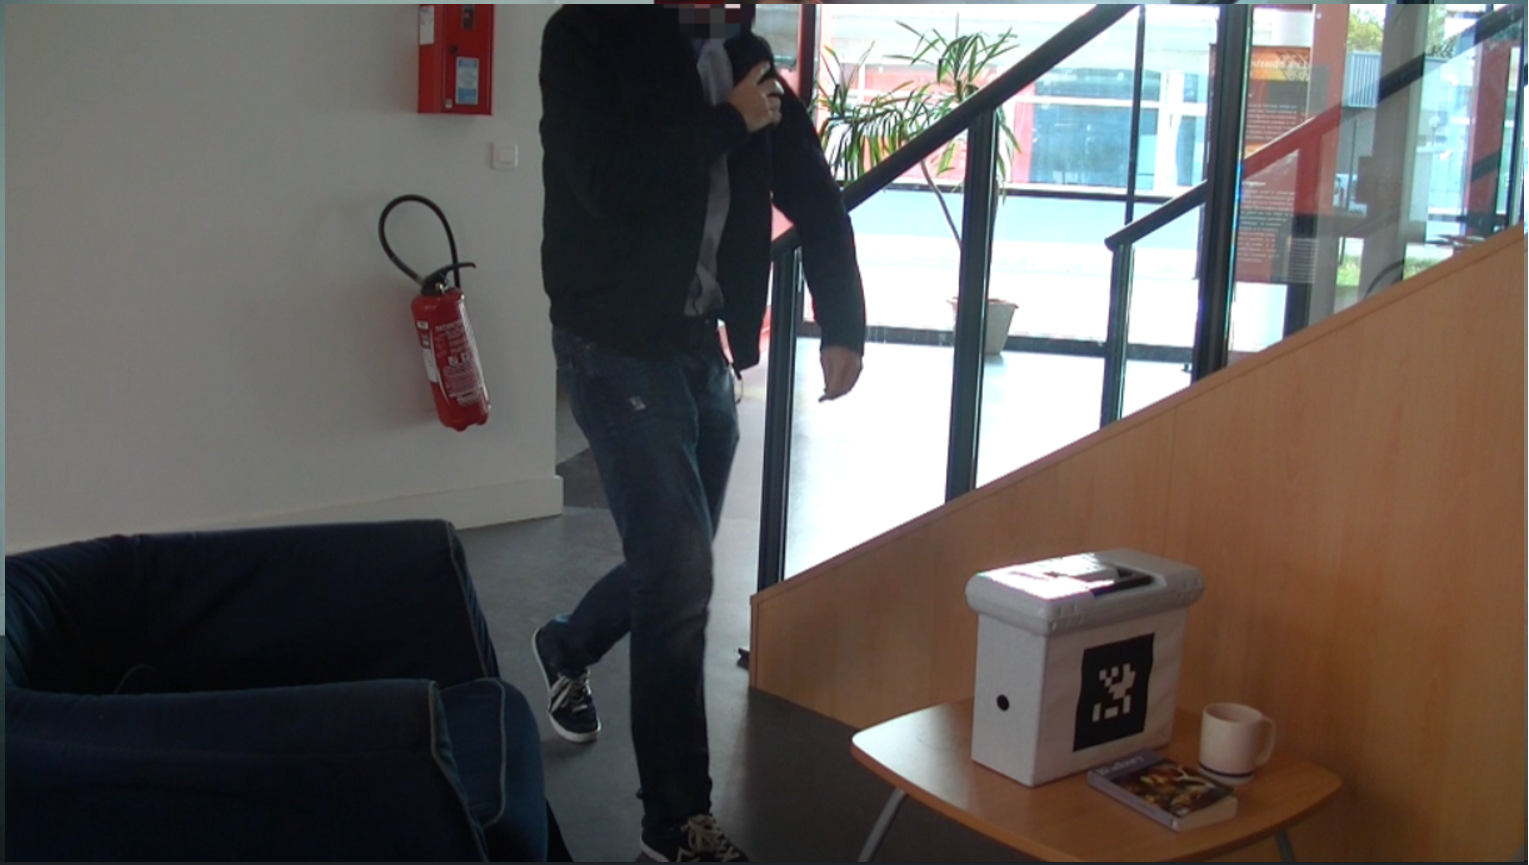
\includegraphics[scale=0.5]{img/observer/keys2-blur.pdf}
	\caption{The keys intention scenario}
	\label{fig:observer_experiments-keys}
\end{figure}

\section{Experiment}
\label{sec:observer_experiment-experiment}
\subsection{User Study}
We built an online user study, where we presented videos related to the tests and events of the two scenarios to users, who had to evaluate the likelihood of each intention of the scenario
on a five-level Likert scale. The user study was conducted in three languages, with users living in two different countries\footnote{A version of this user study was provided at http://goo.gl/forms/YiuFHnF63c}. We collected answers from 78 adults, performed an average, and converted them to percentile scores, in order to compare them with the system's predictions.

Looking at users' answers (figure \ref{fig:observer_experiments-user_study_results}), we can see that, in the absence of clues, people rated similarly the two intentions related to visible objects. Contextual clues had the highest influence on users' ratings. This is particularly visible in the \textit{Contextual Clues} test of the \textit{Keys Scenario}, where users chose as the most likely intention \textit{Take Keys}, even if no keys were visible in the video. Divergent beliefs also influenced users decisions, but not as strongly as context. The strongest responses, over all, where given by the \textit{Divergent Belief Max} test on \textit{Keys Scenario}, which uses both divergent belief and contextual information.

\subsection{System Implementation}
\label{subsec:observer_results-system_implementation}
In this subsection, we show how we implemented this experiment on our system. We will start by showing how we created a simulation of the scenarios. Then we will explain how we computed conditional dependencies between intentions and contexts, and finally we will discuss about the actual implementation of the IGs in the two scenarios.

\subsubsection{Setting up the Simulation}
% At the start of a scenario the robot scanned the environment, building a model of its world state. 
We built a simulation to represent these two scenarios. For each scenario, we set the positions of the objects and computed a starting world state.

 At the start of the scenario, the system does not have information about what each human knows, and so it will assume that they have the same belief model as itself. The system will be able to form a different belief model of each human only with the \textit{Divergent Belief} event. This is a simplification. In the real world, we believe that humans have complex mechanisms to infer others' mental beliefs, based on many aspects. For example, if we would go to the home of a friend, we would probably infer that he has knowledge even about attributes that he can not immediately perceive (e.g. he will know that that he can find a glass in a cabinet in the kitchen even if he can not see it at the moment). Instead, if other people come at our home, we would infer that they do not know where objects are located until they see them. Our system is not able to replicate this idea, leading to our simplification.

 For each test of our simulation, we streamed coordinates related to the body and hand positions of agents, following what was shown in the videos of the user study. For example, if in a test we showed Max moving from the hallway to the table, we streamed a trajectory of coordinates representing this path. 

The inference process was performed by building different IGs for the scenarios. Each test had a different graph, related to its main agent. 

\subsubsection{Contextual Information}
We considered three different Context Nodes for our simulation: \textit{Hot Day}, true when the day is particularly warm; \textit{Break Time}, true when the agents are taking a pause; \textit{Time to Leave}, true when it is late in the day, and the humans usually leave work and return home.

As previously said, we have chosen to follow \cite{Liu2014} in order to learn the link between Context and Intention Nodes. We submitted a questionnaire to 15 users with 16 questions, representing every possible combination of the intentions and contexts used in our scenarios. In each question,
the users had to rate how they perceived that a context influenced a particular intention. The rating was based on a five-level Likert scale, representing the range (\textit{very negatively}, \textit{very positively}). For example, one of the questions asked how a very warm day would influence the probability that the user would drink water.

The conditional dependency between intention $I_i$ and context $C_j$ was computed in the following way: 
\begin{equation}
 P(I_i|C_j=1)=\frac{\sum_{k=1}^5 ncj_k \times v_k}{n\_users}
\end{equation}

where $ncj_k$ is the number of persons who rated the influence of context $C_j$ on intention $I_i$ with the value $k$, $v_k$ is the probability value that we associated to $k$ (where 1=0.1, 2=0.3, 3=0.5, 4=0.7, 5=0.9) and $n\_users=15$ is the number of users that participated in the test.

We set the values of Context Nodes manually in the tests, depending  on the information shown in the videos. While we simulated this aspect, we will give some ideas on how the values of these Context Nodes could be inferred in a real scenario.

\begin{itemize}
\item \textit{Hot Day}. The temperature of the day could be measured by a sensor or obtained from a meteo application. Also, in one of the tests Max is commenting that the day is very warm. A speech recognition software could capture this information.
\item \textit{Break Time} and \textit{Time to Leave}. These information could be either hardcoded (e.g. in the company, workers have an hour of break from 13 to 14 and leave at 17:30) or learnt by observing the agents' activities.
\end{itemize}



\subsubsection{Cookie Scenario}
The starting world state for the cookie scenario is shown in table~\ref{table:observer_results-system_starting_state_cookie}.

 \begin{table}[h!]
\centering
\scriptsize
\renewcommand{\arraystretch}{1.3}
\begin{tabular}{|c|c|}
\hline
MUG isAt TABLE    \\ \hline
BOTTLE isAt TABLE  \\ \hline
COOKIEBOX isAt TABLE   \\ \hline
COOKIEBOX capacity 1    \\ \hline
COOKIES\_SUPPLY isAt KITCHEN    \\ \hline
\end{tabular}
\caption[Starting World State for the Cookie Scenario]{The starting world state for the cookie scenario.}
 \label{table:observer_results-system_starting_state_cookie}    
\end{table}


 With our perception capacities, we would not be able to detect if the cookie box is full or empty, and so we consider it as full (using the attribute $capacity$, which can have a value of 1 or 0) at the start of a test, and update its value using the $postconditions$ of inferred human actions. We consider the box as empty when we infer that a human has taken a cookie from inside, and as full when we infer that a human has put a cookie in it.


In the \textit{Cookie Scenario} the graph for the tests is constructed from the following nodes:
\begin{itemize}
\item Context Nodes: \textit{Hot Day}, \textit{Break Time}, \textit{Time to Leave}
\item Intention Nodes: \textit{Fill Cookie Box}, \textit{Eat Cookie}, \textit{Drink Water}, \textit{Read Book}.
\item Action Nodes: \textit{Move to Table}, \textit{Move to Kitchen}.
\item Observation Nodes: distance of the agent's body and hand to each action's associated \textit{target}.
\end{itemize}

We introduce the \textit{Fill Cookie Box} intention, not present in the human test, to allow the system to detect when Bob fills the \textit{Cookie Box} during the \textit{Divergent Belief Event}.

As previously said, we set Context Nodes to plausible values, that could be extracted by watching the videos. For the \textit{Contextual Clues} test, we set the value of \textit{Hot Day} to true (since Max is commenting about the temperature), and \textit{Break Time} and \textit{Time to Leave} to false (since no data in the video points to one of these contexts being true. Max and Bob seem to have taken a break from work before the other events are shown, in the Divergent Belief Event).

\textit{Divergent Belief Event}, \textit{Divergent Belief No Cookie}, and \textit{Divergent Belief Cookie} were streamed sequentially to the system, which updated the agents' mental models and created new IGs accordingly.
After the \textit{Divergent Belief Event}, the robot inferred that Max has a divergent belief on the \textit{Cookie Box}, because he does not know that Bob filled it. The mental states of the two humans, at this point, is shown in table~\ref{table:observer_results-divergent_event}.


\begin{table}[h!]
\centering
\scriptsize
\renewcommand{\arraystretch}{1.3}
\begin{tabular}{|c|c|}
\hline
Bob & Max \\ \hline \hline
MUG isAt TABLE   & MUG isAt TABLE \\ \hline
BOTTLE isAt TABLE  & BOTTLE isAt TABLE \\ \hline
COOKIEBOX isAt TABLE   & COOKIEBOX isAt TABLE \\ \hline
COOKIEBOX capacity 1  & COOKIEBOX capacity 0   \\ \hline
COOKIES\_SUPPLY isAt KITCHEN & COOKIEBOX\_SUPPLY isAt KITCHEN  \\ \hline
\end{tabular}
\caption[Belief models of Max And Bob after the Divergent Belief Event]{The table shows the belief models of Max and Bob after the Divergent Belief Event. } 
 \label{table:observer_results-divergent_event}    
\end{table}



 During the \textit{Divergent Belief Event} several IGs need to be created with different Action and Observation Nodes, to follow the sequence of actions by the two agents. For example, when \textit{Max} leaves the room, \textit{Bob} has the possibility to execute the actions \textit{Take Mug}, \textit{Take Water Bottle}, \textit{Open Cookie Box}, \textit{Move to Kitchen Shelf} or \textit{Leave Room}. Intention and Context nodes remains the same in all the IGs of the scenario.



\subsubsection{Keys Scenario}
The starting world state for the keys scenario is shown in table~\ref{table:observer_results-system_starting_state_keys}.

 \begin{table}[h!]
\centering
\scriptsize
\renewcommand{\arraystretch}{1.3}
\begin{tabular}{|c|c|}
\hline
BOX isAt TABLE    \\ \hline
BOOK isAt TABLE  \\ \hline
MUG isAt TABLE   \\ \hline
\end{tabular}
\caption[Starting World State for the Keys Scenario]{The starting world state for the keys scenario.}
 \label{table:observer_results-system_starting_state_keys}    
\end{table}

The IG for this scenario is similar to the one for the \textit{Cookie Scenario}, with the following differences.
\begin{itemize}
\item Context Nodes: \textit{Hot Day}, \textit{Break Time} and \textit{Time to Leave}.
\item Intention Nodes: \textit{Drink Water}, \textit{Take Keys}, \textit{Read Book}.
\end{itemize}

Action Nodes and Observation Nodes are the same as the previous scenario, and follow the same ideas during the \textit{Divergent Belief Event}. An example of IG used in the tests can be seen in figure \ref{fig:intention-intention_graph}, presented in chapter~\ref{chapter:intention}. For the \textit{Contextual Clues} and \textit{Divergent Belief} test, we set the \textit{Time to Leave} context value to \textit{true} (since Max is putting on a coat and seems in a hurry), and other Context Node values to \textit{false}. Using the component described in the chapter~\ref{chapter:intention} and these IGs the system was able to obtain predictions from the user actions.

\section{Discussion}
\label{sec:observer_experiment-discussion}
We performed TOST tests for each intention in the scenarios, comparing the humans' answers with the system's, for a total of 21 tests. We calculated p-values and performed our tests using a significance value $\alpha=0.05$.

Analyzing the results of our equivalence tests, shown in figure \ref{fig:observer_experiments-user_study_results}, produces some interesting information.
\begin{itemize}
\item \textbf{The behavior of our system is often close to human capacities}. 16 tests out of 21 passed our requirements   with very low p-value scores. 
\item \textbf{Context and Divergent Belief are necessary}. A system without these skills would only have been able to model properly the \textit{No Clues} cases. 
\item \textbf{There are still some missing aspects in our system}. 
	\begin{itemize}
		\item When our system does not find a strategy to achieve a goal, the probability of the related intention is inferred as zero. Humans, instead, perform a different kind of reasoning. This is particularly evident in the \textit{Contextual Clues} test of the \textit{Keys Scenario}, where our system produced very different results than the users' answers. In this case, contextual information made users think that Max wanted to take the keys, even if no keys where actually present. Somehow, humans are able to infer the mental belief of Max, deducing that maybe he thinks that there are keys on the table. Our system is not able to replicate this reasoning.
		\item In some situations it seems that humans perform complex temporal reasonings. In the \textit{Divergent Belief Cookie} of the \textit{Cookie Scenario}, the users' average answer for the \textit{Eat Cookie} intention was quite high. We believe that users thought that, since Bob, in the previous videos, filled the box, probably he wants to eat a cookie. Contextual information about the warmth of the day where less strong in this case. 
	\end{itemize}

\end{itemize}
 \begin{figure}[ht!]
	\centering
	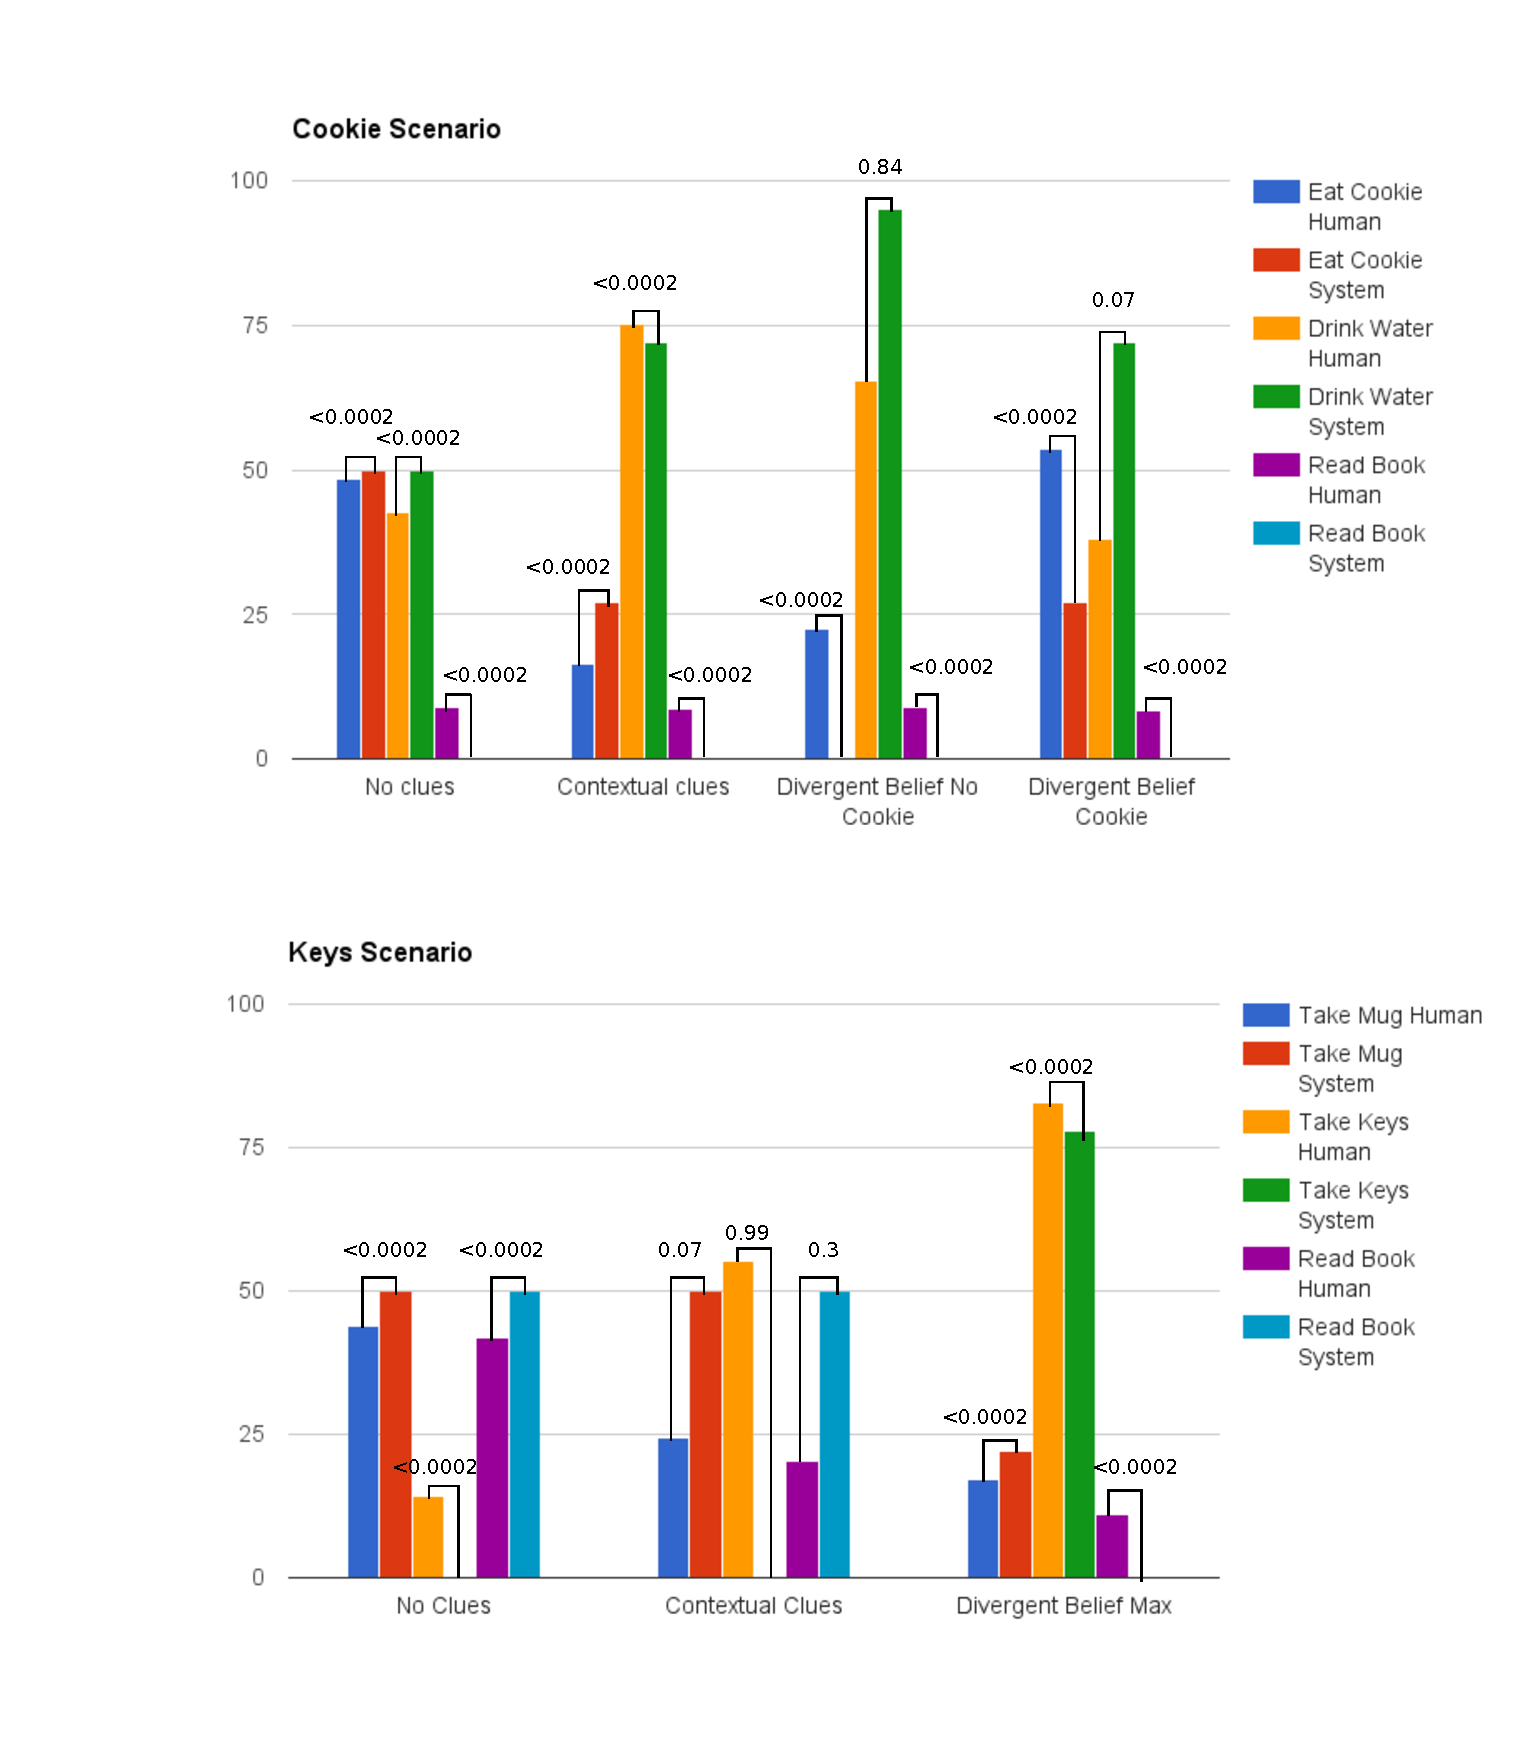
\includegraphics[clip,scale=0.7]{img/observer/scenarios_redone_1.pdf}
	\caption[Experiment results]{Experiment results. Results from the two scenarios are represented as graphs. Intentions, as estimated by the humans and the system, are represented by different colors, as shown in the legend of the graphs, with estimations of the same intention by the system or the human placed in adjacent positions. Each column represents the likelihood of an intention, expressed as a percentile score. P-values from the equivalence tests are shown, linking the estimation of an intention by the humans and by the system.}
	\label{fig:observer_experiments-user_study_results}
\end{figure}



 
